\documentclass[a4paper, 12pt]{./Template/lnls-note-PT}
\usepackage{amsmath}
\usepackage{amsthm}
\usepackage{indentfirst}
\numberwithin{equation}{section} %numera a equação de acordo com sua seção
\usepackage[pdftex,colorlinks=true,citecolor=black,linkcolor=black,urlcolor=black,filecolor=black]{hyperref}
\usepackage[num,abnt-emphasize=bf, bibjustif]{abntex2cite}
\citebrackets[]
%\documentclass[a4paper, 12pt, report]{lnls-note} % if you want to have chapters choose this one

%loads standard preamble configuration
%Standard preamble for documentation preparation

% \usepackage[T1]{fontenc}
% \usepackage{txfonts}
% \usepackage{authblk} % para varios autores em um mesmo artigo
\usepackage{graphicx}
\usepackage{subfigure}
\usepackage{fancyvrb} %fancy verbatim environment
\usepackage{amssymb}  % more symbols
% \usepackage{booktabs}
\usepackage{multirow} % enable multi row in tables
\usepackage{ulem}  % used to strike text
\usepackage{scrextend} % allow reference to footnotes
\usepackage[version=3]{mhchem} % Package for chemical equation typesetting
\usepackage{siunitx} % Package for units in SI
\usepackage{amsmath} % package with several mathematical symbols
% \usepackage{mathtools} % aligned environment inside align environment
% \usepackage[num]{abntcite}
\usepackage{lmodern} % carrega a fonte natural do latex com T1
\usepackage{textcomp} % package with symbols
\usepackage{floatrow}% Table float box with bottom caption, box width adjusted to content
\usepackage[hang,small]{caption}% legendas menores e o hang=alinha a legenda
\usepackage{hyperref} %possibilita o uso das refer�ncias e hiperlinks
\hypersetup{colorlinks,%
	    citecolor=black,%
	    filecolor=black,%
	    linkcolor=black,%
	    urlcolor=blue}
\usepackage{algpseudocode} %algorithmic package
\usepackage{algorithm}     % float environment for algorithm

%loads standard commands
\newcommand{\mc}[3]{\multicolumn{#1}{#2}{#3}} % multicolumns in a table
\newcommand{\mr}[3]{\multirow{#1}{#2}{#3}}    % multirows in a table
\newcommand{\deriva}[2]{\frac{\text{d} #1}{\text{d} #2}} % derivada de #1 em relacao a #2
\newcommand{\bit}{\begin{itemize}}
\newcommand{\eit}{\end{itemize}}
\newcommand{\bce}{\begin{center}}
\newcommand{\ece}{\end{center}}
\newcommand{\beq}{\begin{equation}}
\newcommand{\eeq}{\end{equation}}
\newcommand{\bfl}{\begin{flushleft}}
\newcommand{\efl}{\end{flushleft}}
\newcommand{\degre}{$^\circ$}% Changed this one because there already is a \degree macro in latex
\newcommand{\see}{$\rightarrow$}
\newcommand{\nmrad}{nm$\cdot$rad}
\newcommand{\powten}[1]{$\cdot 10^{#1}$}

\newcommand{\frage}[1]{~\\ \fbox{\small \tt #1}\\}




\begin{document}

\lnlstitle{134518}{\today}{Grupo de Estudos: Física de Aceleradores}
{Isabella Stevani}{\LNLS}
{Seguindo o livro \textit{The physics of electron storage rings: an introdution} de Matthew Sands \cite{sands1970physics}, este grupo de estudos tem por objetivo estudar e discutir o funcionamento de um acelerador de partículas, desde os elementos que o compõe como os fenômenos físicos que modelam sua dinâmica. Este documento traz anotações e deduções úteis de forma a facilitar o completo entendimento deste assunto.}

\newpage
\setcounter{page}{2}
\tableofcontents

\newpage
\section{Introdução}
	\subsection{Comentários iniciais}
    \subsection{Mecanismos básicos}
Para facilitar o entendimento dos processos descritos a seguir, a Figura \ref{fig:ring} representa a estrutura física de um anel de armazenamento.
	
\begin{figure}[!htb]
	\centering
	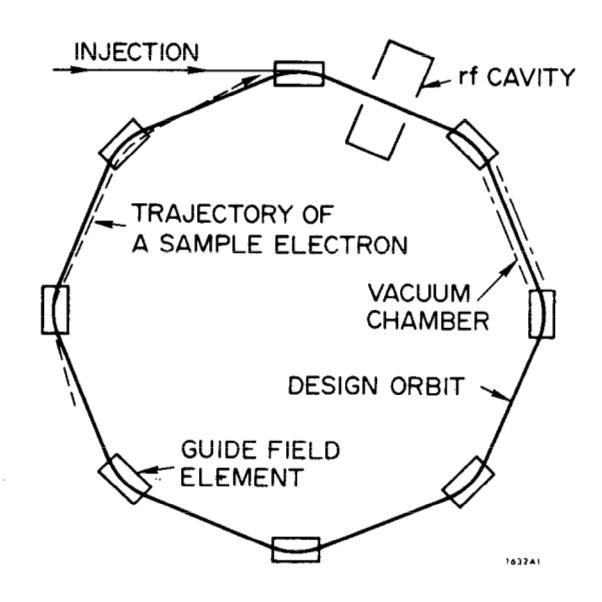
\includegraphics[width=0.6\linewidth]{./Figuras/fig1.jpeg}
	\caption{Diagrama esquemático de um anel de armazenamento de elétrons. Retirado de 						\cite{sands1970physics}.}
	\label{fig:ring}
\end{figure}
	
Um feixe de elétrons é injetado em uma câmara circular em vácuo. Campos magnetostáticos guiam as partículas pela câmara de vácuo. Tais campos são chamados de \emph{campos guia}. A interação eletromagnética entre o campo guia e os elétrons causa uma aceleração centrípeta do feixe, curvando assim sua trajetória e gerando um \emph{órbita fechada} desejada e desenhada a partir da escolha criteriosa do campo.
	
Esse campo guia, além de fechar a trajetória em uma órbita, tem propriedades focalizadoras que fazem com que cada elétron execute oscilações pseudo-harmônicas na transversal, as quais são chamadas de \emph{oscilações betatron}.
	
A cada volta, o elétron perde uma pequena parte da sua energia em forma de \emph{radiação síncrotron}. Esta energia perdida é reposta através de campos elétricos oscilantes no tempo gerados na \emph{cavidade de rádio frequência} (RF) e que aceleram longitudinalmente o feixe. Essas pequenas variações de perda e ganho da energia dos elétrons causam também oscilações no comprimento de órbita, no período de revolução, e ainda, no instante de chegada $\tau$ dos elétrons na cavidade de RF. As oscilações no plano energia-$\tau$ são chamadas de \emph{oscilações síncrotron} (ou oscilações de fase). Essas oscilações longitudinais dos elétrons são medidas em relação às \emph{partículas síncronas}, que são definidas como aqueles elétrons idealizados cujas energias, períodos de revolução e fase de chegada à cavidade de RF têm valores nominais.

Existem fases ideais de chegada à cavidade de RF em que o campo elétrico da cavidade é tal que a energia reposta por ele coincide com a energia média perdida pelos elétrons em cada volta. Cada uma destas fases ideais é chamada de \emph{fase síncrona}. O \emph{número harmônico} de um anel é definido como sendo a razão inteira entre a frequência de RF e a frequência de revolução dos elétrons. O número harmônico nos dá então o número de fases síncronas que podem ser acomodados no anel. Ao redor de cada uma destas fases síncronas, que são pontos fixos do espaço de fase energia-$tau$ nos quais se situam as partícula síncronas, pode-se ter uma distribuição de elétrons descrevendo oscilações síncrotron. Estas distribuições de elétrons em torno de das fases síncronas são chamadas de pacotes ou \emph{bunches}. Tipicamente o número harmônico dos anéis assume valor alto, permitindo assim um grande número de bunches e, em consequência, uma corrente de feixe circulante mais intensa.
	
A perda de energia por radiação síncrotron junto com a compensação gerada pela cavidade de RF causa um lento amortecimento da radiação de todas as amplitudes de oscilação, fazendo com que a trajetória de cada elétron tenda à trajetória do elétron de referência, o qual possui velocidade constante ao longo da órbita ideal.
	
Amortecimento da radiação não conserva o espaço de fase, então pode-se injetar vários \textit{bunches} no mesmo anel. O amortecimento de todas as amplitudes de oscilação é efetivamente preso devido à excitação contínua das oscilações por um "ruído" na energia do elétron, que vem do fato da radiação síncrona ser emitida em fótons de energia discreta. Este fenômeno é chamado de flutuação quântica da perda de energia. Em condições estacionárias, um equilíbrio é alcançado entre a excitação quântica e o amortecimento da radiação, levando a uma distribuição estatística estacionária das amplitudes e fases de oscilação dos elétrons em um \textit{bunch}. O \textit{bunch}, então, toma forma de uma tira elástica viajante, a qual tem tamanho e forma estacionários, com uma distribuição Gaussiana das amplitudes em cada coordenada transversal e longitudinal (Figura \ref{fig:fig2}). 
	
\begin{figure}[!htb]
	\centering
	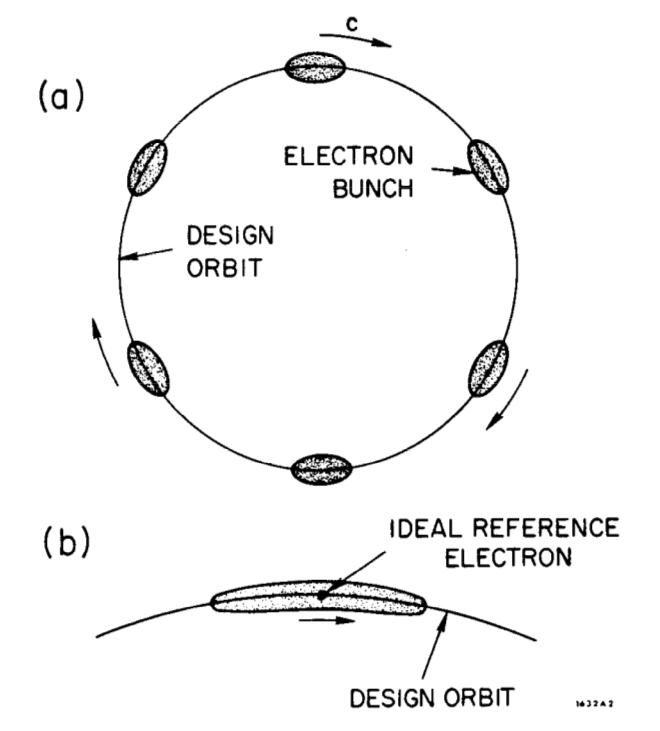
\includegraphics[width=0.55\linewidth]{./Figuras/fig2.jpeg}
	\caption{\textit{Bunches} circulando em um anel de armazenamento. Retirado de 							\cite{sands1970physics}.}
	\label{fig:fig2}
\end{figure}
	
Para cada coordenada do elétron, existe uma amplitude de oscilação máxima chamada de abertura dinâmica, a qual o elétron não fica mais preso dentro do \textit{bunch}. A abertura dinâmica para cada coordenada é definida por um obstáculo físico (tamanho da câmara de vácuo, por exemplo) ou por efeitos não-lineares nas forças focalizadoras, gerando trajetórias não-limitadas.
    \subsection{Efeitos coletivos}
Quando há um número suficientemente grande de elétrons em um \textit{bunch}, as interações entre os elétrons são relevantes (seja entre os elétrons ou entre os \textit{bunches}). 
	
\begin{itemize}
	\item \textit{Touschek-effect}. Dois elétrons oscilando em um \textit{bunch} podem transferir um pouco da sua energia de oscilação de uma coordenada transversal para uma longitudinal se sofrerem espalhamento de Coulomb. As novas amplitudes podem estar fora da aceitância em energia, ou aumentar o tamanho do \textit{bunch}. Esse efeito é relevante em baixas energias (menor que 1 GeV).
    \item Oscilações coerentes. Cada elétron no feixe produz campos eletromagnéticos na câmara de vácuo 	que influenciam o movimento dos outros elétrons. Estas interações coletivas podem gerar oscilações 		coerentes instáveis, em que todos os elétrons de um \textit{bunch} oscilam num modo coletivo em que 	a amplitude aumenta exponencialmente com o tempo. Estas oscilações coerentes envolvem tanto a 			dinâmica transversal quanto a longitudinal, podendo aumentar o tamanho do \textit{bunch} ou levar à 	perda de elétrons.
\end{itemize}
	
Interferência construtiva dos campos de radiação dos elétrons em um \textit{bunch} talvez gere radiação síncrona coerente, que pode aumentar a perda de energia de cada elétron individualmente. Este efeito não é considerado significante nos anéis de armazenamento mais novos.
	
Para conseguir a alta densidade de corrente desejada nos anéis de armazenamento, as instabilidades coerentes devem ser suprimidas ou controladas. Os outros efeitos coletivos são combinados com os efeitos individuais para determinar a dimensão do \textit{bunch}.
    \pagebreak
  
\section{Oscilações Betatron}
	\subsection{Sistema de coordenadas}
É conveniente utilizar um sistema de coordenadas cilíndrico para descrever a trajetória de um elétron dentro do anel de armazenamento (\autoref{fig:fig7}), uma vez que é desejado que seu movimento seja circular. Sendo assim, definem-se as coordenadas
\begin{itemize}
	\item $s$ -- Coordenada longitudinal, representa a distância entre um ponto de referência na órbita ideal e o ponto mais próximo do elétron nesta mesma órbita.
	\item $x$ e $z$ -- Coordenadas transversais, representam os deslocamentos horizontal e vertical com relação à órbita ideal, respectivamente.
\end{itemize}

\begin{figure}[!htb]
	\centering
	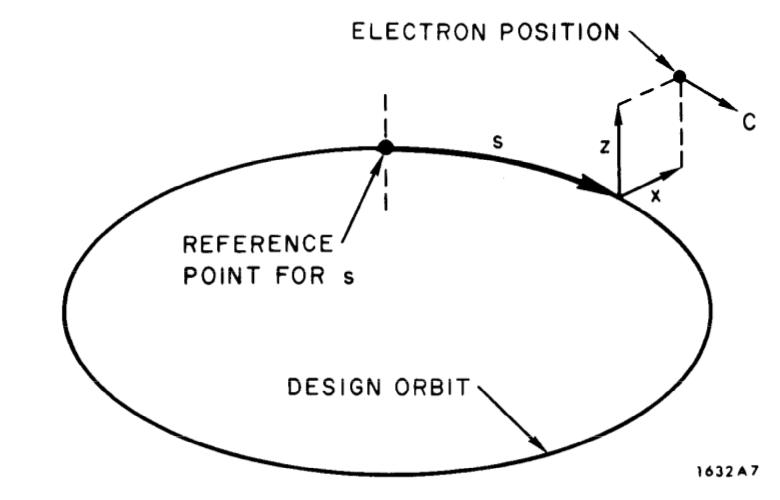
\includegraphics[width=0.6\linewidth]{./Figuras/fig7.jpeg}
	\caption{Coordenadas para descrever as trajetórias. Retirado de \cite{sands1970physics}.}
	\label{fig:fig7}
\end{figure}
    \subsection{Campo guia}\label{sec:2.2}
Pelo principio da inércia de Newton, um corpo tende a permanecer em movimento retilínio uniforme se não há forças que o obriguem a mudar sua trajetória. Logo, para que o elétron tenha uma órbita circular, é necessário aplicar uma força que mude sua trajetória da forma desejada.

Pela força de Lorentz,
\begin{align}
	\vec{F} = q\left(\vec{E} + \vec{v} \times \vec{B}\right)
\end{align}
onde $q$ é a carga da partícula em movimento, $\vec{E}$ é o vetor de campo elétrico, $\vec{v}$ é o vetor de velocidade da partícula e $\vec{B}$ é o vetor de campo magnético.

A contribuição referente à força elétrica ($q\vec{E}$) é paralela ao campo elétrico, enquanto a contribuição referente à força magnética ($q(\vec{v}\times\vec{B})$) é perpendicular ao campo magnético e à velocidade. Devido a este fato, a força magnética não realiza trabalho, uma vez que é perpendicular ao deslocamento da partícula. Logo, a força magnética altera a direção do vetor velocidade -- e, por consequência, do movimento da partícula -- sem alterar o seu módulo. Apenas a força elétrica pode realizar trabalho.

Desta forma, a fim de desviar a partícula da sua trajetória, aplica-se um campo magnético $\vec{B}$ nos pontos onde ela deve fazer alguma curva, o qual é chamado de campo guia. Com $E=0$,
\begin{align}
	\vec{F} = q\vec{v}\times\vec{B}
\end{align}

Espera-se que a órbita ideal ocorra no plano horizontal ($z=0$) de forma que o campo magnético deve ser puramente vertical em toda a órbita do anel. Considerando o campo magnético simétrico com relação ao plano da órbita ideal e fazendo uma aproximação linear, pode-se escrever a equação do campo magnético através da expansão de Taylor:
\begin{align}
	B_z(s,x,z) &= B_0(s) + \left(\frac{\partial B_z}{\partial x}\right)_{0s} x\label{eq:2.01}\\
	B_x(s,x,z) &= \left(\frac{\partial B_x}{\partial z}\right)_{0s} z\label{eq:2.02}
\end{align}

Pela simetria imposta, aplicando as leis de Maxwell,
\begin{align}
	\frac{\partial B_z}{\partial x} = \frac{\partial B_x}{\partial z}
\end{align}

Desta forma, as equações \eqref{eq:2.01} e \eqref{eq:2.02} podem ser reescritas como
\begin{align}
	B_z(s,x,z) &= B_0(s) + \left(\frac{\partial B}{\partial x}\right)_{0s} x\label{eq:2.1}\\
	B_x(s,x,z) &= \left(\frac{\partial B}{\partial x}\right)_{0s} z\label{eq:2.2}
\end{align}

Como o campo é simétrico em relação ao plano da órbita ideal, as variáveis $B_0$ e $\frac{\partial B}{\partial x}$ possuem apenas componentes verticais, então apenas suas magnitudes são necessárias para descrevê-las completamente e os índices $s$ e $z$ podem ser suprimidos.

Anéis de armazenamento são modelados para operar em uma faixa de valores de energia dos elétrons. Isto é obtido arranjando de forma que os campos magnéticos possam ser variados juntos -- sendo parametrizados proporcionalmente à energia de operação desejada. Claramente, se o campo magnético na órbita ideal é mudado em todo o anel pelo mesmo fator, a órbita ideal será, novamente, uma trajetória possível de um elétron cujo momento é mudado pelo mesmo fator. Variar todos os campos juntos altera muito pouco a energia associada com a órbita ideal. Por essas razões, é conveniente especificar as propriedades do campo guia de uma maneira que seja independente de qualquer energia de operação escolhida, o que é facilmente feito dividindo todos os campos por um fator proporcional à energia associada do elétron, o qual é chamado de rigidez magnética. Desta forma, as propriedades lineares do campo guia podem ser definidas pelas funções
\begin{align}
	G(s) &= \frac{ecB_0(s)}{E_0}\label{eq:2.3}\\
	K_1(s) &= \frac{ec}{E_0} \left(\frac{\partial B}{\partial x}\right)_{0s}
\end{align}
onde $E_0$ é a energia nominal, $c$ é a velocidade da luz e $e$ é a carga do elétron. Note que estas funções tem um significado físico bem simples. Neste caso, apenas elétrons ultra-relativísticos são considerados, então sua energia é dada por $E=cp$. Desta forma, $G(s)$ é apenas o inverso do raio de curvatura $\varrho(s)$ dos elétrons em $x=0$ e $z=0$ com energia nominal, ou seja,
\begin{align}
	G(s) = \frac{1}{\varrho(s)}
\end{align}

\begin{proof}
	Como a partícula está rotacionando sobre ação da força de Lorentz, esta força deve ser equivalente a sua força centrípeta. Logo,
	\begin{align*}
		\frac{mv^2}{\varrho(s)} &= q\vec{v}\times\vec{B}\\
							    &= evB_0(s)\\
	\end{align*}
	
	Como o elétron é ultra-relativístico (com velocidade próxima/igual à velocidade da luz), a energia da partícula é dada por
	\begin{align*}
		E_0^2 = (m_0 c^2)^2 + p^2c^2
	\end{align*}
	onde $m_0$ é a massa de repouso e $p$ o momento da partícula. Pelo mesmo argumento anterior, $(m_0c^2)^2 << c^2p^2$. Desta forma, pode desprezar o termo $(m_0c^2)^2$ e a energia da partícula é dada por
	
	\begin{align*}
		E_0 &= pc\\
			&= \gamma m_0 c^2\\
			&= mc^2
	\end{align*}
	
	Substituindo,
	\begin{align*}
			\frac{mv^2}{\varrho(s)} &= ecB_0(s)\\
			\frac{E_0}{\varrho(s)} &= ecB_0(s)\\
			\therefore \frac{1}{\varrho(s)} &= \frac{ecB_0(s)}{E_0} = G(s)
	\end{align*}
	
	Desta forma, reescrevendo a equação do campo magnético em função de $G(s)$,
	\begin{align*}
		B_z(s,x,z) &= B_0(s) + \frac{\partial B}{\partial x} x\\
				   &= \frac{E_0}{ec} G(s) + \frac{\partial B}{\partial x} x
	\end{align*}
	
	Definindo a função $K_1(s)$ como
	\begin{align*}
		K_1(s) = \frac{ec}{E_0} \frac{\partial B}{\partial x}
	\end{align*}
	tem-se que
	\begin{align*}
		B_z(s,x,z) &= \frac{E_0}{ec} G(s) + \frac{\partial B}{\partial x} x\\
				   &= \frac{E_0}{ec} G(s) + \frac{E_0}{ec} K_1(s) x\\
				   &= \frac{E_0}{ec} [G(s) + K_1(s) x]
	\end{align*}
	Reescrevendo $B_x(s,x,z)$ da mesma forma, as equações do campo magnético são
	\begin{align*}
		B_z(s,x,z) &= \frac{E_0}{ec} [G(s) + K_1(s) x]\\
		B_x(s,x,z) &= \frac{E_0}{ec} K_1(s) z
	\end{align*}
\end{proof}

A constante de proporcionalidade $\frac{E_0}{ec}$ é a rigidez magnética do anel de armazenamento. Ela normaliza as equações do campo magnético de forma que este dependa apenas das propriedades da ótica do anel.

Devido à relação entre $G(s)$ e $\varrho(s)$, $G(s)$ é chamada de função de curvatura. A função $K_1(s)$ é a taxa de variação do raio inverso com o deslocamento radial.

As funções $G(s)$ e $K_1(s)$ podem ser arbitrárias, porém devem satisfazer alguns requisitos importantes. Primeiro, $G(s)$ precisa ser tal que esta defina uma órbita fechada (pode-se pensar que $G(s)$ define a órbita ideal, ou que alguma órbita fechada arbitrária define $G(s)$ de forma única). A variação $d \theta_0$ na direção da tangente à órbita ideal em um intervalo $ds$ é
\begin{align}
	-d\theta_0 = \frac{ds}{\varrho(s)} = G(s)ds
\end{align}

O ângulo percorrido em uma revolução precisa ser igual a $2\pi$, então $G(s)$ deve satisfazer
\begin{align}
	\int_{0}^{L} G(s)ds = 2\pi
\end{align}

Segundo, tanto $G(s)$ quanto $K_1(s)$ são, necessariamente, funções periódicas de $s$, devido ao fato de que a coordenada longitudinal $s$ é fisicamente cíclica -- retornando ao mesmo ponto da órbita após uma revolução. Dito isso, $G(s)$ e $K_1(s)$ também devem satisfazer
\begin{align}
	\left\{\begin{array}{rcl}
	\ G(s+L) & = & G(s)\\
	K_1(s+L) & = & K_1(s)
	\end{array}\right.
\end{align}
onde $L$ é o comprimento da órbita. Execeto por estas condições, $G(s)$ e $K_1(s)$ podem ter mais ou menos variações arbitrárias com $s$.

Apesar das funções do campo guia $G$ e $K_1$ serem, a princípio, bem gerais, geralmente é conveniente simplificar o design ou a operação de um anel de armazenamento impondo certas restrições nestes aspectos. Por exemplo, a maioria dos anéis de armazenamento são desenhados para ter o mesmo raio de curvatura, diga-se $\varrho_0$, em todos os ímãs de curvatura -- e sem nenhuma curvatura entre um ímã e outro, ou seja, apenas trechos retos. Este tipo de campo guia é chamado isomagnético. O intuito desta configuração é que o campo magnético sobre a órbita ideal tenha o mesmo valor em todo lugar, exceto onde este é nulo. Então $G(s)$ é uma função dicotômica:
\begin{align}
	G(s) = \left\{\begin{array}{rrrr}
	\ G_0 & = & \frac{1}{\varrho_0}, &  no\ \acute{i}m\tilde{a}\\
	0, & & & em\ todo\ o\ resto
	\end{array}\right.
\end{align}

Um campo guia real não pode, claro, ser idealmente isomagnético, já que é fisicamente impossível ter um campo magnético descontínuo. Sempre há uma zona de transição nas bordas do ímã onde o campo vai de zero ao seu valor nominal. A aproximação isomagnética ideal é, entretanto, um tanto quanto adequada no geral.

Apesar de aceleradores e anéis de armazenamento comumente serem construídos com ímãs de curvatura com gradientes radiais de campo, é comum desenvolver campos guia de função separável, ou seja, campos magnéticos em que as funções de focalização e curvatura são atribuídas a elementos magnéticos diferentes. Isto é, o campo guia consiste numa sequência de dipolos (sem gradiente de campo) e quadrupolos (sem campo na órbita ideal). Pensando nesta configuração, define-se um campo guia de função separável onde as funções $G(s)$ e $K_1(s)$ devem satisfazer a condição
\begin{align}
	G(s)K_1(s) = 0\label{eq:2.10}
\end{align}

Um pouco de atenção para este fato. Às vezes é conveniente projetar os ímãs de curvatura com faces retangulares. Com este tipo de ímã, a órbita ideal deve entrar ou sair do ímã com um ângulo diferente de 90$^\circ$ em relação à borda do mesmo (Figura \ref{fig:fig8}). Mesmo que o ímã seja plano (sem gradiente radial no ímã), irão existir gradientes radiais nas bordas, onde o campo não é nulo. A equação \eqref{eq:2.10} não é satisfeita nas bordas, e um campo guia construído com estes ímãs retangulares -- junto com os quadrupolos -- não irá satisfazer a definição de função separável, mesmo que ele seja referenciado como tal às vezes. Estes campos ainda podem ser, entretanto, isomagnéticos. 

\begin{figure}[!htb]
	\centering
	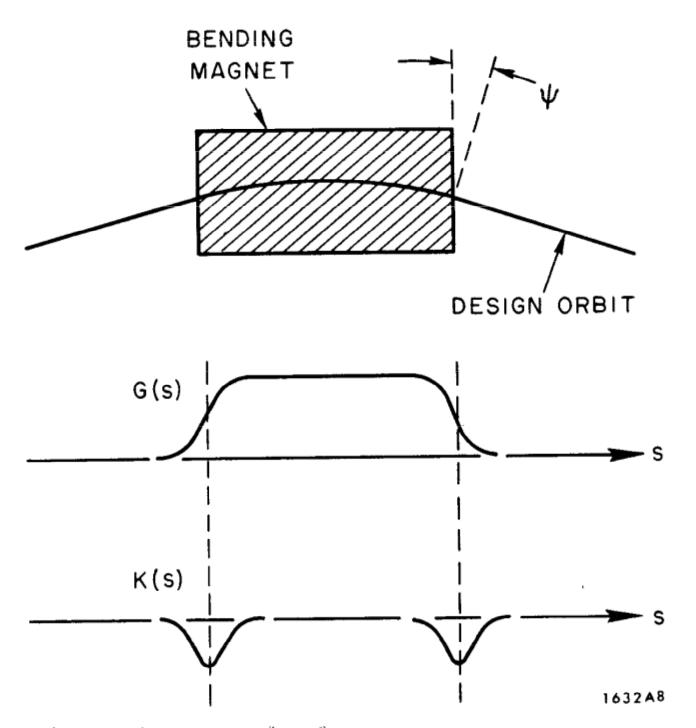
\includegraphics[width=0.6\linewidth]{./Figuras/fig8.jpeg}
	\caption{Campo guia com ímã retangular. Retirado de \cite{sands1970physics}.}
	\label{fig:fig8}
\end{figure}
    \subsection{Equações de movimento}\label{sec:2.3}
As equações de movimento descrevem a trajetória de um elétron se movendo próximo da órbita ideal, com uma energia próxima, mas não necessariamente igual, à energia nominal $E_0$. O desvio de energia é definido como
\begin{align}
	\epsilon = E-E_0
\end{align}
onde $E$ é a energia do elétron.

Para manter a aproximação linear, são considerados apenas pequenas quantidades de $x$, $z$ e $\epsilon$. Melhor do que tomar o tempo como variável independente, é mais conveniente adotar a coordenada longitudinal $s$. Assim, derivadas com relação a $s$ serão indicadas daqui pra frente pela notação $(')$. Por exemplo, $x'=\frac{dx}{ds}$.

Começando a análise pelo movimento radial. Considere um elétron em $x$ movendo-se com inclinação $x'$ (Figura \ref{fig:fig9}). A inclinação é o ângulo entre a direção do movimento do elétron e a tangente à órbita ideal. $x'$ é o ângulo entre a trajetória e a tangente à órbita ideal. Suponha um ângulo $\theta_0$ entre a tangente e uma direção de referência arbitrária e um ângulo $\theta$ entre a trajetória e a mesma direção de referência. Logo, $x' = \theta-\theta_0$ e
\begin{align}
	x'' = \frac{d(\theta-\theta_0)}{ds}\label{eq:2.12}
\end{align}

\begin{figure}[!htb]
	\centering
	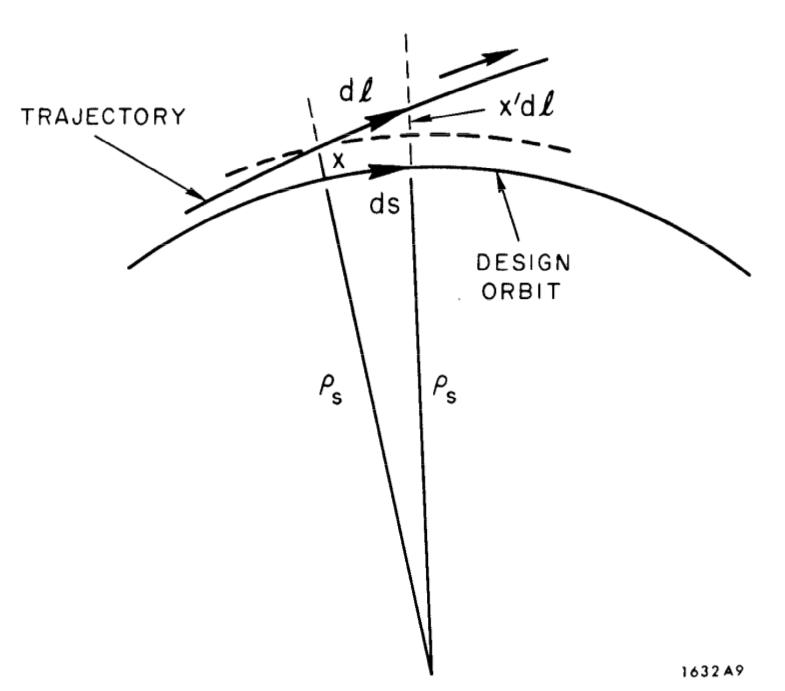
\includegraphics[width=0.6\linewidth]{./Figuras/fig9.jpeg}
	\caption{Trajetória de um elétron próxima à órbita ideal. Retirado de \cite{sands1970physics}.}
	\label{fig:fig9}
\end{figure}

A derivada de $\theta_0$ é, como já foi visto, $\frac{-1}{\varrho_s} = G(s)$ ($\varrho_s = \varrho(s)$). Mas o que é $\frac{d\theta}{ds}$? O rario de curvatura da trajetória é
\begin{align}
	\varrho = \frac{E}{ecB}
\end{align}
e, em um elemento de caminho $d\ell$ da trajetória, a variação do ângulo é
\begin{align}
	d\theta = -\frac{d\ell}{\varrho} = -\frac{ecB}{E}d\ell\label{eq:2.14}
\end{align}

Note que, enquanto o ângulo $x'$ é pequeno -- e pode-se sempre assumir isto desde que apenas termos de primeira ordem sejam considerados, que é o caso -- um elemento de caminho $d\ell$ da trajetória em $x$ é relacionado com a correspondente variação em $s$ por
\begin{align}
	d\ell = \frac{\varrho_s - x}{\varrho_s} ds = \left(1+\frac{x}{\varrho_s}\right)ds = (1+G(s))ds\label{eq:2.15}
\end{align}

Agora, $B$ pode ser descrito por
\begin{align}
	B = B_0 + \frac{\partial B}{\partial x}x = \frac{E_0}{ec}(G+K_1x)\label{eq:2.16}
\end{align}

Substituindo as equações \eqref{eq:2.15} e \eqref{eq:2.16} na equação \eqref{eq:2.14} juntamente com $E_0+\epsilon$ para $E$ -- e mantendo apenas termos de primeira ordem -- tem-se que
\begin{align}
	d\theta = \left\{-G-(G^2+K_1)x + G\frac{\epsilon}{E_0}\right\}ds
\end{align}
e, portanto, 
\begin{align}
	x'' = -(G^ 2+K_1)x + G\frac{\epsilon}{E_0}
\end{align}

\begin{proof}
	Pela equação \eqref{eq:2.14},
	\begin{align*}
		d\theta &= -\frac{ecB}{E}d\ell\\
				&= -\frac{ecB}{E}(1+Gx)ds\\
				&= -\frac{ec}{E}\left[\frac{E_0}{ec}(G+K_1x)\right](1+Gx)ds\\
				&= -\frac{E_0}{E_0+\epsilon}(G+K_1x)(1+Gx)ds\\
				&= -\frac{E_0}{E_0+\epsilon}(G+K_1x+G^2x+K_1Gx^2)ds\\
				&= -\frac{E_0}{E_0+\epsilon}(G+(G^2+K_1)x + K_1Gx^2)ds
	\end{align*}
	
	Mantendo apenas termos de primeira ordem para continuar com a aproximação linear,
	\begin{align*}
		d\theta &= -\frac{E_0}{E_0+\epsilon}(G+(G^2+K_1)x)ds\\
				&= \frac{E_0}{E_0+\epsilon}(-G-(G^2+K_1)x)ds\\
				&= \frac{1}{1+\epsilon/E_0}(-G-(G^2+K_1)x)ds\\
	\end{align*}
	
	Como $\epsilon/E_0$ é bem pequeno, pode-se considerar que o termo $\frac{1}{1+\epsilon/E_0}$ é a soma de uma série geométrica. Logo, pode-se expandir este termo em um somatório:
	\begin{align*}
		d\theta &= \left(1 - \frac{\epsilon}{E_0} + \frac{\epsilon^2}{E_0^2}+ ...\right)(-G-(G^2+K_1)x)ds
	\end{align*}
	
	Novamente, mantendo apenas termos de primeira ordem,
	\begin{align*}
		d\theta &= \left(1 - \frac{\epsilon}{E_0}\right)(-G-(G^2+K_1)x)ds\\
				&= (-G-(G^2+K_1)x)ds + \left(G\left(\frac{\epsilon}{E_0}\right)+(G^2+K_1)x\left(\frac{\epsilon}{E_0}\right)\right)ds
	\end{align*}
	
	Aplicando novamente o argumento acima,
	\begin{align*}
		d\theta = \left\{-G-(G^2+K_1)x + G\frac{\epsilon}{E_0}\right\}ds
	\end{align*}
	
	Agora, pela equação \eqref{eq:2.12},
	\begin{align*}
		x'' &= \frac{d(\theta-\theta_0)}{ds}\\
			&= \frac{\left\{-G-(G^2+K_1)x + G\frac{\epsilon}{E_0}\right\}ds - (-G)ds}{ds}\\
			&= -(G^2+K_1)x + G\frac{\epsilon}{E_0}
	\end{align*}
\end{proof}

A equação correspondente para o movimento vertical é
\begin{align}
	z'' = K_1 z
\end{align}

\begin{proof}
	Para $z''$, pela força de Lorentz,
	\begin{align*}
		d\theta &= -\frac{d\ell}{\varrho} = + \frac{ecB}{E}d\ell\\
				&= \frac{ecB}{E}d\ell\\
				&= \frac{ecB}{E}(1+Gx)ds\\
				&= K_1 z (1+Gx)ds\\
				& = (K_1 z + GK_1xz)ds
	\end{align*}
	
	Descartando o termo de segunda ordem,
	\begin{align*}
		d\theta &= K_1 z ds\\
	\end{align*}
	
	Agora, pela equação \eqref{eq:2.12},
	\begin{align*}
		z'' &= \frac{d(\theta-\theta_0)}{ds}\\
			&= \frac{K_1 z\ ds}{ds}\\
			&= K_1 z
	\end{align*}
	lembrando que $\frac{d\theta_0}{ds} = 0$ porque não há componente vertical nesta variação.
\end{proof}

Definindo as funções focalizadoras $K_x$ e $K_z$ como
\begin{align}
	K_x(s) &= G^2(s)+K_1(s)\label{eq:2.21}\\
	K_z(s) &= - K_1(s)
\end{align}
tem-se que $x''$ e $z''$ podem ser descritos como
\begin{align}
	x'' &= -K_x(s)x + G(s)\frac{\epsilon}{E_0}\label{eq:2.19}\\
	z'' &= -K_z(s)z\label{eq:2.20}
\end{align}

O termo correspondente à $G^2$ está "faltando" de $K_z$ devido à consideração de que a órbita ideal está no plano, ou seja, não possui componente vertical. Mais especificamente, $G^2$ é um termo de força centrífuga, e um termo correspondente apareceria no movimento vertical se a órbita tivesse picos e vales. Anéis de armazenamento possuem, em geral, uma forte focalização. Neste caso, $G^2$ é bem menor que $K_1$, então $K_x$ e $K_z$ são aproximadamente iguais e possuem sinais opostos. Fisicamente, esta diferença de sinal significa que um elemento focalizador que focaliza em $x$ automaticamente desfocaliza em $z$, e vice-versa.

A equação de movimento em $z$ parece a equação de uma oscilação clássica (força proporcional ao desvio), com um coeficiente de força restauradora variável -- a função $K_z(s)$. A equação em $x$ é similar, exceto pela adição de um termo variável proporcional ao desvio de energia $\epsilon$. Nos campos guia que podem ser efetivamente utilizados, as soluções destas equações são, na verdade, oscilatórias, e descrevem oscilações laterais -- incluindo as chamadas oscilações betatron -- na trajetória do elétron. Estas oscilações são resultado das propriedades focalizadoras do campo guia, as quais caracterizam as funções de focalização $K_x$ e $K_z$.

Tanto $K_x$ quanto $K_z$ são funções periódicas ao longo do anel, logo
\begin{align}
	\begin{array}{rcl}
	\ K(s+L) & = & K(s)
	\end{array}
\end{align}

Por conveniência na construção e no design do anel, este possui uma periodicidade intrínseca. Ou seja, é composta por uma sequência de células magnéticas idênticas, cada célula sendo constituída por dipolos e quadrupolos. Então, para um anel com células de comprimento $\ell_c$,
\begin{align}
	\left\{\begin{array}{rcl}
	\ G(s+\ell_c) & = & G(s)\\
	K(s+\ell_c) & = & K_1(s)
	\end{array}\right.
\end{align}

Nota-se que, diferentemente da primeira propriedade, a periodicidade de célula é uma propriedade do design da máquina, não sendo totalmente verdadeira em campos reais devido a imperfeições na construção.

Na \autoref{fig:fig10}, a natureza das funções de focalização em uma parte do anel, abrangendo duas células. A Figura \ref{fig:fig10} (a) mostra o configuração dos dipolos e quadrupolos do anel. Os dipolos são denominados por B e tem um campo uniforme ($dB/dx = 0$). Os quadrupolos não tem campo na órbita ideal ($B_0=0$) e são denominados por F e D (F para focalizador e D para desfocalizador, ambos com relação ao movimento radial). As Figuras \ref{fig:fig10} (b) e (c) são as funções de focalização $G$, $K_x$ e $K_z$.

\begin{figure}[!htb]
	\centering
	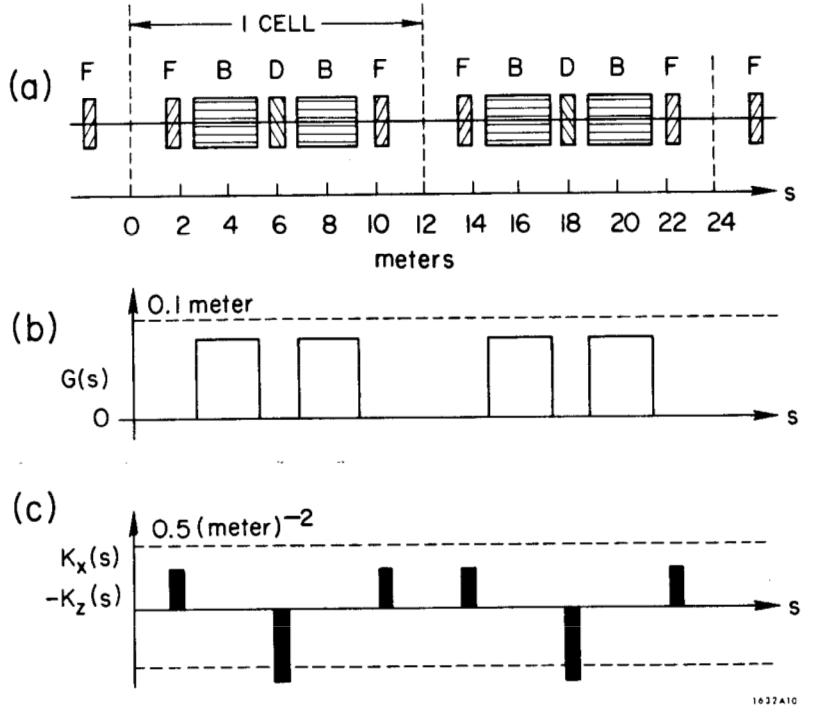
\includegraphics[width=0.7\linewidth]{./Figuras/fig10.jpeg}
	\caption{Laço magnético e funções de focalização em uma célula de um campo guia em particular. Retirado de \cite{sands1970physics}.}
	\label{fig:fig10}
\end{figure}
    \subsection{Separação do movimento radial}
É conveniente separar o movimento radial em duas partes: uma parte sendo uma curva fechada deslocada da órbita de design -- a órbita de equilíbrio dos elétrons com desvio de energia -- e a outra parte sendo a oscilação transversal em torno desta órbita. Suponha que $x$ seja
	
\begin{align}
	x = x_{\epsilon} + x_{\beta}\label{eq:2.25}
\end{align}
então certamente a equação \eqref{eq:2.19} é satisfeita se as equações
\begin{align}
	x_\epsilon'' &= -K_x(s)x_\epsilon + G(s)\frac{\epsilon}{E_0}\label{eq:2.26}\\
	x_\beta'' &= -K_x(s)x_\beta\label{eq:2.27}
\end{align}
forem verdadeiras.
	
\begin{proof}
    Pela equação \eqref{eq:2.25}, $x = x_{\epsilon} + x_{\beta}$. Logo,
    \begin{align*}
        x'' &= x_{\epsilon}'' + x_{\beta}''\\
            &= -K_x(s)x_\epsilon + G(s)\frac{\epsilon}{E_0} + K_x(s)x_\beta\\
            &= -K_x(s)(x_\epsilon + x_\beta) + G(s)\frac{\epsilon}{E_0}\\
            &= -K_x(s)x + G(s)\frac{\epsilon}{E_0}
    \end{align*}
\end{proof}
	
Definindo que $x_\epsilon(s)$ é uma função periódica em $s$ com período $L$, então $x_\epsilon(s)$ é a órbita fechada de um elétron com energia $E_0 + \epsilon$ (com $x_\beta=0$), e o movimento radial será a soma do desvio dessa nova órbita de equilíbrio e uma oscilação betatron.
	
O desvio $x_\epsilon$ é proporcional ao desvio de energia $\epsilon$. Define-se	
\begin{align}
	x_\epsilon(s) = \eta(s)\frac{\epsilon}{E_0}\label{eq:2.29}
\end{align}
onde $\eta(s)$ é a função única que satisfaz	
\begin{align}
	\begin{cases}
		\eta'' = -K_x(s)\eta + G(s), \\
        \eta(0) = \eta(L), \\
        \eta'(0) = \eta'(L).
    \end{cases}
\end{align}
	
\begin{proof}
	Seja $x_\epsilon(s)$ dado pela equação \eqref{eq:2.29}. Pela equação \eqref{eq:2.26},
	\begin{align*}
        x_\epsilon'' &= -K_x(s)x_\epsilon + G(s)\frac{\epsilon}{E_0}\\
        \left(\eta(s)\frac{\epsilon}{E_0}\right)'' &= -K_x(s)\eta(s)\frac{\epsilon}{E_0} + G(s)\frac{\epsilon}{E_0}\\
        \eta(s)''\frac{\epsilon}{E_0} &= -K_x(s)\eta(s)\frac{\epsilon}{E_0} + G(s)\frac{\epsilon}{E_0}\\
        \eta'' &= -K_x(s)\eta + G(s)
	\end{align*}
\end{proof}
	
Denomina-se $\eta(s)$ como sendo a função de órbita fechada, e é uma função que caracteriza o campo guia total do anel. Note que $\eta (s)$ é a solução particular da equação diferencial \eqref{eq:2.26} em que a função é periódica com período $L$ e não depende de características do elétron, apenas da ótica do anel.
    \subsection{Trajetórias betatron}\label{sec:2.5}
As equações \eqref{eq:2.20} e \eqref{eq:2.27} descrevem as oscilações betatron vertical e radial, respectivamente. Considerando as aproximações feitas, o movimento em cada coordenada é independente. Logo, como $K_x(s)$ e $K_z(s)$ tem a mesma forma matemática, toma-se a forma representativa
	
\begin{align}
	x'' = -K(s) \; x \label{eq:2.31}
\end{align}
	
Lembrando que $K_x(s)$ descreve a oscilação betatron radial de um elétron com energia nominal $E_0$ e $K_z(s)$ descreve o movimento vertical.
	
A função de focalização $K(s)$ é definida em cada coordenada $s$ pelo design do anel de armazenamento. Se a posição e a inclinação ($x$ e $x'$) são dadas em alguma coordenada $s$, os termos subsequentes podem ser obtidos integrando a equação \eqref{eq:2.31}. Porém, como o campo guia é construído de segmentos magnéticos e $K(s)$ pode ser considerada constante nestes intervalos, pode-se integrar $x$ e $x'$ para cada segmento e juntar estes resultados. Dependendo do valor de $K$, $x$ é dado por

\begin{align}
	\left\{\begin{array}{l}
	K>0: \ \ x = a\ \cos(\sqrt{K}s+b) \\
	K=0: \ \ x = as+b \\
	K<0: \ \ x = a\ \cosh(\sqrt{-K}s+b)
	\end{array}\right. \label{eq:2.32}
\end{align}
onde $a$ e $b$ são constantes em cada segmento e podem ser determinadas pelos valores de $x$ e $x'$ na entrada do segmento (como $K$ é finita em qualquer ponto, $x$ e $x'$ devem ser ambas contínuas em todo ponto -- em particular, na junção entre dois segmentos).
	
\begin{proof}
	A equação \eqref{eq:2.31} é uma equação diferencial homogênea de 2ª ordem. Considerando que a função $K$ é uma constante, supõe-se que a solução da EDO é uma exponencial, 		ou seja, da forma $x=e^{rs}$. Substituindo esta possível solução, tem-se
	\begin{align*}
		x'' + Kx &=0\\
		(e^{rs})'' + K(e^{rs}) &= 0\\
		r^2e^{rs} + Ke^{rs}&=0\\
		(r^2 + K)e^{rs} &=0\\
		e^{rs} \neq 0 \therefore r^2 + K &= 0
	\end{align*}
	
	A equação $r^2 + K = 0$ é a equação característica da EDO. Resolvendo-a, tem-se $r = \pm \sqrt{-K}$, então $x_{1,2} = e^{\pm\sqrt{-K}s}$. Agora, existem 3 casos possíveis:
	\begin{itemize}
		\item $K>0$\\
			
		Com $K<0$, as raízes da equação característica são imaginárias. A solução geral da EDO é, para este caso, $x = c_1e^{\alpha s}\cos(\beta s) + c_2e^{\alpha s}\sin(\beta s)$. Como a função seno é apenas a função cosseno com uma diferença de fase, pode-se escrever
        \begin{align*}
        	x = a \ \cos(\sqrt{K}+b)
        \end{align*}
			
		\item $K = 0$\\
		
		A solução geral da EDO é, para este caso, $x = c_1e^{\sqrt{K}s} + sc_2e^{-\sqrt{K}s}$. Como $K=0$, 
		\begin{align*}
            x &= c_1e^{\sqrt{K}s} + sc_2e^{\sqrt{K}s}\\
            x &= c_1e^{0s} + sc_2e^{0s}\\
            x &= c_1 + sc_2
		\end{align*}
		
		Renomeando as constantes, $x = as + b$.

		\item $K < 0$\\
				
		A solução geral da EDO é, para este caso, $x = c_1e^{\sqrt{-K}s} + c_2e^{-\sqrt{-K}s}$. Fazendo $c_1=c_2=\frac{1}{2}$,
		\begin{align*}
            x &= c_1e^{\sqrt{-K}s} + c_2e^{-\sqrt{-K}s}\\
            x &= \frac{e^{\sqrt{-K}s} + e^{-\sqrt{-K}s}}{2} = cosh(\sqrt{-K}x)
		\end{align*}
				
		Para constantes $c_1$ e $c_2$ arbitrárias,
		\begin{align*}
          x = a \ cosh(\sqrt{-K}x + b)
		\end{align*}
	\end{itemize}
	
	Concluindo,
	\begin{align*}
        \left\{\begin{array}{l}
        K>0: \ \ x = a\ \cos(\sqrt{K}s+b) \\
        K=0: \ \ x = as+b \\
        K<0: \ \ x = a\ \cosh(\sqrt{-K}s+b)
        \end{array}\right.
	\end{align*}
\end{proof}

Como ilustração, supõe-se uma funçãoi $K(s)$ como a função $K_x(s)$ na \autoref{fig:fig10}. Duas possíveis trajetórias estão representadas na \autoref{fig:fig11} (b). A primeira é a trajetória que começa em $s_0$ com deslocamento unitário $x_0=1$ e nenhuma inclinação $x_0'=0$. A segunda começa com deslocamento nulo $x_0=0$ e inclinação unitária $x_0'= 1$. A primeira é chamada de \textit{cosinelike trajectory} -- $C$ e a segunda de \textit{sinelike trajectory} -- $S$. Seus detalhes dependem da coordenada de referência $s_0$ e são, em geral, funções não periódicas, mesmo que $K(s)$ seja. Para um anel com trajetórias estáveis, $C$ e $S$ são funções oscilatórias limitadas as quais possuem uma forma diferente a cada revolução.

\begin{figure}[!htb]
	\centering
	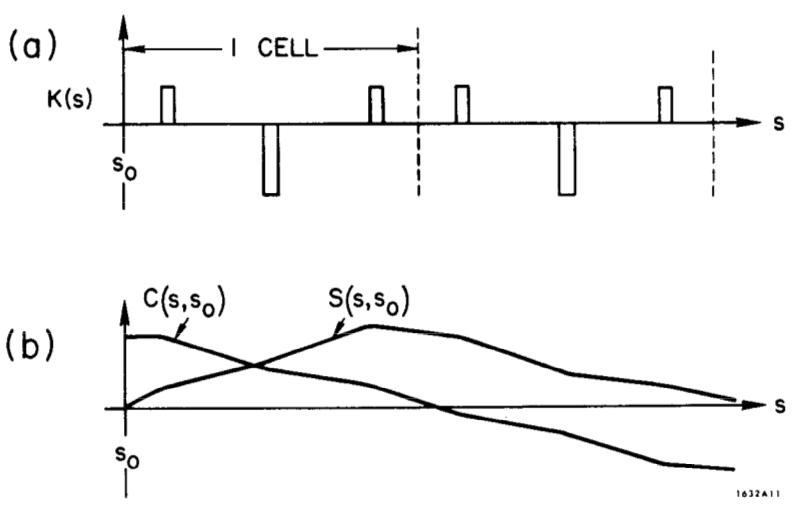
\includegraphics[width=0.7\linewidth]{./Figuras/fig11.jpeg}
	\caption{Função de focalização $K(s)$ e duas trajetórias: a \textit{cosine-like trajectory} e a \textit{sine-like trajectory} para uma coordenada de início $s_0 $. Retirado de \cite{sands1970physics}.}
	\label{fig:fig11}
\end{figure}
	
Agora, como a equação \eqref{eq:2.31} é linear em $x$, qualquer combinação linear de $C$ e $S$ também descreve uma trajetória possível para $x$. Mais que isso, qualquer trajetória pode ser descrita por esta combinação linear. Ou seja,
	
\begin{align}
	x(s) &= C(s,s_0)x_0 + S(s,s_0)x_0'\\
	x'(s) &= C'(s,s_0)x_0 + S'(s,s_0)x_0'
\end{align}
onde $C'$ e $S'$ são as derivadas de $C$ e $S$ em relação a $s$ e $x_0$ e $x_0'$ são os valores de $x$ e $x'$ em $s_0$. É conveniente escrever esta equação na forma matricial:
	
\begin{align}
	\boldsymbol{x}(s)=\boldsymbol{M}(s,s_0)\boldsymbol{x}(s_0)
\end{align}
onde 
\begin{align}
	\boldsymbol{x}(s) = \begin{bmatrix}
	x(s)\\ 
	x'(s)
	\end{bmatrix}
\end{align}
e
\begin{align}
	\boldsymbol{M}(s,s_0) = \begin{bmatrix}
	C(s,s_0) & S(s,s_0)\\
	C'(s,s_0) & S'(s,s_0)
	\end{bmatrix}\label{eq:2.37}
\end{align}
	
$\boldsymbol{M}(s,s_0)$ é a matriz de transferência de $s_0$ para $s$, a qual depende apenas de propriedades do campo guia entre duas coordenadas. A matriz de transferência de um trecho pode ser obtida em termos das matrizes de segmentos deste trecho. Logo, para um $s_1$ entre $s$ e $s_0$,
	
\begin{align}
	\boldsymbol{M}(s,s_0) = \boldsymbol{M}(s,s_1)\boldsymbol{M}(s_1,s_0)
\end{align}
	
\begin{proof}
	Pela definição da equação \eqref{eq:2.37},
	\begin{align*}
        \boldsymbol{M}(s,s_1) = \begin{bmatrix}
        C(s,s_1) & S(s,s_1)\\
        C'(s,s_1) & S'(s,s_1)
        \end{bmatrix}
	\end{align*} e
    \begin{align*}
		\boldsymbol{M}(s_1,s_0) = \begin{bmatrix}
		C(s_1,s_0) & S(s_1,s_0)\\
		C'(s_1,s_0) & S'(s_1,s_0)
		\end{bmatrix}
	\end{align*}
	
	Logo,
	\begin{align*}
        \boldsymbol{M}(s,s_0) &= \boldsymbol{M}(s,s_1)\boldsymbol{M}(s_1,s_0)\\
        &= \begin{bmatrix}
            C(s,s_1) & S(s,s_1)\\
            C'(s,s_1) & S'(s,s_1)
            \end{bmatrix} \begin{bmatrix}
                               C(s_1,s_0) & S(s_1,s_0)\\
                              C'(s_1,s_0) & S'(s_1,s_0)
                              \end{bmatrix}\\
        &= \begin{bmatrix}
        C(s,s_1)C(s_1,s_0)+S(s,s_1)C'(s_1,s_0) & C(s,s_1)S(s_1,s_0) + S(s,s_1)S'(s_1,s_0)\\
        C'(s,s_1)C(s_1,s_0)+S'(s,s_1)C'(s_1,s_0) & C'(s,s_1)S(s_1,s_0) + S'(s,s_1)S'(s_1,s_0)
        \end{bmatrix}	
	\end{align*}
	
	Considerando que $s_1 = s+\Delta_1$ e $s_0 = s_1 + \Delta_0$, então $(s,s_1) = \Delta_1$ e $(s_1,s_0) = \Delta_0$. Como $s_1$ é um ponto entre $s$ e $s_0$, também tem-se que $(s,s_0) = \Delta_1 + \Delta_0$. Logo, 
	\begin{align*}
        \boldsymbol{M}(\Delta_1)\boldsymbol{M}(\Delta_0) &= \begin{bmatrix}
        C(\Delta_1)C(\Delta_0)+S(\Delta_1)C'(\Delta_0) & C(\Delta_1)S(\Delta_0) + S(\Delta_1)S'(\Delta_0)\\
        C'(\Delta_1)C(\Delta_0)+S'(\Delta_1)C'(\Delta_0) & C'(\Delta_1)S(\Delta_0) + S'(\Delta_1)S'(\Delta_0)
        \end{bmatrix}
	\end{align*}
	
	Sabendo que $S'=C$ e $C'=-S$,
	\begin{align*}
        \boldsymbol{M}(\Delta_1)\boldsymbol{M}(\Delta_0) &= \begin{bmatrix}
        C(\Delta_1)C(\Delta_0)-S(\Delta_1)S(\Delta_0) & C(\Delta_1)S(\Delta_0) + S(\Delta_1)C(\Delta_0)\\
        -S(\Delta_1)C(\Delta_0)-C(\Delta_1)S(\Delta_0) & -S(\Delta_1)S(\Delta_0) + C(\Delta_1)C(\Delta_0)
        \end{bmatrix}
	\end{align*}
	
	Por propriedades trigonométricas,
	\begin{align*}
        [\boldsymbol{M}(\Delta_1)\boldsymbol{M}(\Delta_0)]_{11} &= \frac{1}{2}[C(\Delta_1-\Delta_0)+C(\Delta_1+\Delta_0)] - \frac{1}{2}[C(\Delta_1-\Delta_0)-C(\Delta_1+\Delta_0)]\\
        [\boldsymbol{M}(\Delta_1)\boldsymbol{M}(\Delta_0)]_{12} &= \frac{1}{2}[S(\Delta_1+\Delta_0)-S(\Delta_1-\Delta_0)] + \frac{1}{2}[S(\Delta_1-\Delta_0)+S(\Delta_1+\Delta_0)]\\
        [\boldsymbol{M}(\Delta_1)\boldsymbol{M}(\Delta_0)]_{21} &= -\frac{1}{2}[S(\Delta_1-\Delta_0)+S(\Delta_1+\Delta_0)] - \frac{1}{2}[S(\Delta_1+\Delta_0)-S(\Delta_1-\Delta_0)]\\
        [\boldsymbol{M}(\Delta_1)\boldsymbol{M}(\Delta_0)]_{22} &= -\frac{1}{2}[C(\Delta_1-\Delta_0)-C(\Delta_1+\Delta_0)] + \frac{1}{2}[C(\Delta_1-\Delta_0)+C(\Delta_1+\Delta_0)]
	\end{align*}
	
	Simplificando os termos da matriz, tem-se
	\begin{align*}
        \boldsymbol{M}(\Delta_1)\boldsymbol{M}(\Delta_0) &= \begin{bmatrix}
        C(\Delta_1+\Delta_0) & S(\Delta_1+\Delta_0)\\
        -S(\Delta_1+\Delta_0) & C(\Delta_1+\Delta_0)
        \end{bmatrix}\\
        &= \begin{bmatrix}
            C(\Delta_1+\Delta_0) & S(\Delta_1+\Delta_0)\\
            C'(\Delta_1+\Delta_0) & S'(\Delta_1+\Delta_0)
            \end{bmatrix}\\
        \boldsymbol{M}(s,s_1)\boldsymbol{M}(s_1,s_0)&= \begin{bmatrix}
            C(s,s_0) & S(s,s_0)\\
            C'(s,s_0) & S'(s,s_0)
            \end{bmatrix} = \boldsymbol{M}(s,s_0) 
	\end{align*}
	c.q.d.
\end{proof}
	
Para os três casos possíveis de $K$ descritos na equação \eqref{eq:2.32},
	
\begin{align}
	K>0: \ \ \boldsymbol{M}(s_2,s_1) &= \begin{bmatrix}
	\cos(\sqrt{K}\ell) & \frac{1}{\sqrt{K}}\ sen(\sqrt{K}\ell)\\
	-\sqrt{K}\ sen(\sqrt{K}\ell) & \cos(\sqrt{K}\ell)
	\end{bmatrix}\\
	K=0: \ \ \boldsymbol{M}(s_2,s_1) &= \begin{bmatrix}
		1 & \ell\\
		0 & 1
		\end{bmatrix}\\
	K<0: \ \ \boldsymbol{M}(s_2,s_1) &= \begin{bmatrix}
		\cosh(\sqrt{-K}\ell) & \frac{1}{\sqrt{-K}}\ senh(\sqrt{-K}\ell)\\
		\sqrt{-K}\sinh(\sqrt{-K}\ell) & \cosh(\sqrt{-K}\ell)
		\end{bmatrix}
\end{align}
onde $\ell = s_2-s_1$.
	
\begin{proof}Analisando para os três casos de $K$:
	\begin{itemize}
	\item $K>0$\\
	
	Da equação \eqref{eq:2.32}, tem-se que $C(s_2,s_1) = \cos(\sqrt{K}\ell)$. Logo,
	\begin{align*}
        C'(s_2,s_1) &= \frac{d\ \cos(\sqrt{K}\ell)}{d\ell} = -\sqrt{K}\sin(\sqrt{K}\ell)\\
        S(s_2,s_1) &= \int \cos(\sqrt{K}\ell)d\ell = \frac{1}{\sqrt{K}}\sin(\sqrt{K}\ell)\\
        \therefore \boldsymbol{M}(s_2,s_1) &= \begin{bmatrix}
            \cos(\sqrt{K}\ell) & \frac{1}{\sqrt{K}}\ sen(\sqrt{K}\ell)\\
            -\sqrt{K}\ sen(\sqrt{K}\ell) & \cos(\sqrt{K}\ell)
            \end{bmatrix}
	\end{align*}
	\item $K=0$\\
	
	Da equação \eqref{eq:2.32}, tem-se que $C(s_2,s_1) = 1$. Logo,
	\begin{align*}
		C'(s_2,s_1) &= \frac{d \ 1}{d\ell} = 0\\
		S(s_2,s_1) &= \int d\ell = \ell\\
		\therefore \boldsymbol{M}(s_2,s_1) &= \begin{bmatrix}
				1 & \ell\\
				0 & 1
				\end{bmatrix}
	\end{align*}
	\item $K<0$\\
	
	Da equação \eqref{eq:2.32}, tem-se que $C(s_2,s_1) = \cosh(\sqrt{-K}\ell)$. Logo,
		\begin{align*}
        	C'(s_2,s_1) &= \frac{d\ \cosh(\sqrt{-K}\ell)}{d\ell} = \sqrt{-K}senh(\sqrt{-K}\ell)\\
            S(s_2,s_1) &= \int \cosh(\sqrt{-K}\ell)d\ell = \frac{1}{\sqrt{-K}}senh(\sqrt{-K}\ell)\\
            \therefore \boldsymbol{M}(s_2,s_1) &= \begin{bmatrix}
            \cosh(\sqrt{-K}\ell) & \frac{1}{\sqrt{-K}}\ senh(\sqrt{-K}\ell)\\
            \sqrt{-K}\ senh(\sqrt{-K}\ell) & \cosh(\sqrt{-K}\ell)
            \end{bmatrix}
		\end{align*}
	\end{itemize}
\end{proof}
	
A solução geral da equação \eqref{eq:2.31} pode ser escrita como
	
\begin{align}
	x(s) = a\zeta(s)\ cos\{\varphi(s)-\vartheta\}\label{eq:2.39}
\end{align}
onde $\zeta(s)$ e $\varphi(s)$ são funções especialmente definidas em $s$ com certas propriedades convenientes, e $a$ e $\vartheta$ são constantes obtidas pelas condições iniciais, as quais determinam uma trajetória particular. Define-se
	
\begin{align}
	\varphi(s) = \int_{0}^{s} \frac{d\bar{s}}{\zeta^2(\bar{s})}
\end{align}
	
Então
\begin{align}
	\varphi'(s) = \frac{1}{\zeta^2}
\end{align}
e, se $\zeta(s)$ for definida para ser essa função positiva, analítica que satisfaz
\begin{align}
	\zeta'' = -K(s)\zeta+\frac{1}{\zeta^3}\label{eq:2.41}
\end{align}
então $x(s)$ da equação \eqref{eq:2.39} satisfaz a equação diferencial \eqref{eq:2.31}.
	
\begin{proof}
	Seja $x(s)$ dado pela equação \eqref{eq:2.39}. Então,
	\begin{align*}
        x' &= [a\zeta\ \cos\{\varphi-\vartheta\}]'\\
        &= a[\zeta'\cos(\varphi-\vartheta)-\zeta\varphi'\sin(\varphi-\vartheta)]\\
        \therefore x'' &= a[\zeta'\cos(\varphi-\vartheta)-\zeta\varphi'\sin(\varphi-\vartheta)]'\\
        &= a\left[\zeta''\cos(\varphi-\vartheta)-\zeta'\varphi'\sin(\varphi-\vartheta) - \left(-\frac{\zeta'}{\zeta^2}\sin(\varphi-\vartheta)+\frac{\varphi'}{\zeta}\cos(\varphi-\vartheta)\right)\right]
	\end{align*}
	
	Pela equação \eqref{eq:2.41}, 
	\begin{align*}
        x'' &= a\left[\left(-K\zeta+\frac{1}{\zeta^3}\right)\cos(\varphi-\vartheta)-\frac{\zeta'}{\zeta^2}\sin(\varphi-\vartheta) + \frac{\zeta'}{\zeta^2}\sin(\varphi-\vartheta)-\frac{1}{\zeta^3}\cos(\varphi-\vartheta)\right]\\
        &= -Ka\zeta\ \cos(\varphi-\vartheta)\\
        &= -Kx
	\end{align*}
	
	Assim, pode-se ver que $x(s) = a\zeta(s)\ \cos\{\varphi(s)-\vartheta\}$ é solução da equação diferencial \eqref{eq:2.31}.
\end{proof}
	
Tradicionalmente, define-se a função betatron $\beta(s)$ como
\begin{align}
	\beta(s) = \zeta^2(s)
\end{align}
então
\begin{align}
	x(s) &= a\sqrt{\beta(s)}\ \cos\{\varphi(s)-\vartheta\}\label{eq:2.43}\\
	\varphi(s) &= \int_{0}^{s} \frac{d\bar{s}}{\beta(\bar{s})}\label{eq:2.44}
\end{align}
	
Note que, dada a função de focalização $K(s)$ do anel, $\beta(s)$ pode ser unicamente determinada. Porém, enquanto $K(s)$ é dada em função das propriedades locais do campo guia, a função $\beta(s)$ -- ou $\zeta(s)$ depende da configuração total do anel. Por outro lado, uma vez que $\beta(s)$ é conhecida, $K(s)$ pode ser imediatamente determinada pelas suas derivadas locais, mas é $\beta(s)$ que revela de forma mais direta as características significantes da trajetória dos elétrons armazenados.
	
Lembrando que toda a discussão feita nesta subsseção se aplica tanto no movimento radial quanto no vertical, ou seja, o anel é descrito pelas funções $\beta_x$ e $\beta_z$, as quais são derivadas das funções de focalização $K_x$ e $K_z$, respectivamente.
    \subsection{Oscilações betatron pseudo-harmônicas}
As equações \eqref{eq:2.43} e \eqref{eq:2.44} descrevem completamente o caminho realizado pelo elétron. Para ter uma visão completa do movimento do elétron, basta apenas adicionar o fato de que o elétron viaja sempre na velocidade $c$ da luz. Fazendo uma aproximação, é adequado tomar que a coordenada longitudinal $s$ varia simplesmente como
	
\begin{align}
	s = s_0 + ct\label{eq:2.48}
\end{align}
	
A forma correta da equação \eqref{eq:2.48} será discutida na Seção \ref{sec:3.2}.
	
A função betatron descreve completamente as propriedades laterais de focalização do campo guia. Pela sua natureza, a função betatron deve ser sempre positiva definida, e sua curva tem uma forma semelhante a uma onda. Ela também é periódica ao longo do anel, logo
	
\begin{align}
	\beta(s+L) = \beta(s)
\end{align}
	
A função betatron possui um valor único em cada coordenada $s$. Se o campo guia é dividido em células idênticas (desconsiderando imperfeições de construção), $\beta$ terá a mesma simetria.
	
Conforme o elétron viaja ao redor do anel, ele executa uma oscilação lateral que não é nem harmônica e nem periódica. O movimento é um tipo de onda senoidal (\ref{fig:fig12}) distorcida com uma amplitude $a\sqrt{\beta}$ variante, a qual é modulada proporcionalmente à raiz da função betatron e com uma fase $(\varphi-\upsilon)$ que avança com $s$ a uma taxa de variação proporcional a $\frac{1}{\beta}$.
	
\begin{figure}[!htb]
	\centering
	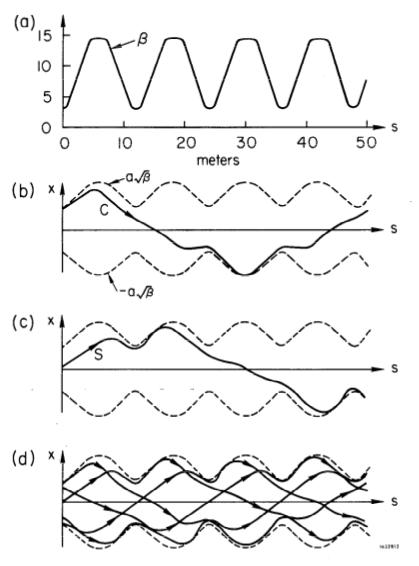
\includegraphics[width=0.7\linewidth]{./Figuras/fig12.jpeg}
	\caption{(a) Função betatron. (b) \textit{Cosine-like trajectory} para $s=0$. (c) \textit{Sine-like trajectory} para $s=0$. (d) Uma trajetória depois de várias revoluções sucessivas. Retirado de \cite{sands1970physics}.}
	\label{fig:fig12}
\end{figure}
	
Uma importante propriedade do movimento betatron é evidente na \ref{fig:fig12}(d) -- em cada coordenada, o desvio $x$ de um elétron em movimento fica sempre abaixo de um valor limitante $X(s)$, o qual é obtido colocando $cos(\varphi-\upsilon)=1$, ou seja,
	
\begin{align}
	X(s) = a\sqrt{\beta(s)}
\end{align}
	
A trajetória completa de um elétron armazenado cairá sempre dentro de um envelope definido por $\pm X(s)$. Segue que a abertura necessária para conter um elétron com uma amplitude de oscilação que varia ao redor do anel varia como $X(s)$. A relação entre a largura do envelope em duas coordenadas $s_1$ e $s_2$ é
	
\begin{align}
	\frac{X_2}{X_1} = \sqrt{\frac{\beta_2}{\beta_1}}
\end{align}
	
Para analisar a inclinação da trajetória betatron, ou seja, $x'=\frac{dx}{ds}$, considera-se a derivada da equação \eqref{eq:2.43}:
	
\begin{align}
	x' = - \frac{a}{\sqrt{\beta}}sen(\varphi-\upsilon)+\frac{\beta'}{2\beta}x\label{eq:2.52}
\end{align}
	
O primeiro termo vem da mudança de fase, e o segundo da variação de $\beta$.
	
\begin{proof}
	Seja $x(s) = a\sqrt{\beta(s)}\ cos\{\varphi(s)-\upsilon\}$. Logo, 
	\begin{align*}
      x' &= [a\sqrt{\beta}\ cos\{\varphi-\upsilon\}]'\\
         &= a[(\sqrt{\beta})'cos(\varphi-\upsilon)-\sqrt{\beta}\varphi'sen(\varphi-\upsilon)]\\
      	 &= a\left[\frac{\beta'}{2\sqrt{\beta}}cos(\varphi-\upsilon)-\sqrt{\beta}\frac{1}{\beta}sen(\varphi-\upsilon)\right]\\
      	 &= a\left[\frac{\beta'}{2\sqrt{\beta}}cos(\varphi-\upsilon)-\frac{1}{\sqrt{\beta}}sen(\varphi-\upsilon)\right]\\
      	 &= \frac{\beta'}{2\sqrt{\beta}}a\ cos(\varphi-\upsilon)-\frac{a}{\sqrt{\beta}}sen(\varphi-\upsilon)\\
      	 &= \frac{\beta'}{2\beta}a\sqrt{\beta}\ cos(\varphi-\upsilon)-\frac{a}{\sqrt{\beta}}sen(\varphi-\upsilon)\\
      	 &= -\frac{a}{\sqrt{\beta}}sen(\varphi-\upsilon)+\frac{\beta'}{2\beta}x
	\end{align*}
\end{proof}
	
Note que os zeros de $x'$ -- e, portanto, os valores de pico de $x$ -- não ocorrem em $cos(\varphi-\upsilon)=1$. Eles ocorrem em
	
\begin{align}
	tg(\varphi-\upsilon) = \frac{\beta'}{2}
\end{align}
o que significa que
\begin{align}
	cos(\varphi-\upsilon) = \left[1+\frac{\beta'^2}{4}\right]^{-\frac{1}{2}}
\end{align}
	
\begin{proof}
	Fazendo $x'=0$:
	\begin{align*}
        x'&=0\\
        -\frac{a}{\sqrt{\beta}}sen(\varphi-\upsilon)+\frac{\beta'}{2\beta}x &= 0\\
        \frac{\beta'}{2\beta}x &= \frac{a}{\sqrt{\beta}}sen(\varphi-\upsilon)\\
        \frac{\beta'}{2\beta}a\sqrt{\beta}\ cos\{\varphi-\upsilon\} &= \frac{a}{\sqrt{\beta}}sen(\varphi-\upsilon)\\
        \frac{\beta'}{2\beta}\sqrt{\beta}\sqrt{\beta} &= \frac{a}{a}\frac{sen(\varphi-\upsilon)}{cos(\varphi-\upsilon)}\\
        \frac{\beta'}{2} &= tg(\varphi-\upsilon)
	\end{align*}
	
	Pela identidade trigonométrica $1+tg^2(x) = sec^2(x)$,
	\begin{align*}
        1+tg^2(\varphi-\upsilon) &= sec^2(\varphi-\upsilon)\\
        1+\left(\frac{\beta'}{2}\right)^2 &= \left(\frac{1}{cos(\varphi-\upsilon)}\right)^2\\
        1+\frac{\beta'^2}{4} &= \frac{1}{cos^2(\varphi-\upsilon)}\\
        cos^2(\varphi-\upsilon) &= \left[1+\frac{\beta'^2}{4}\right]^{-1}\\
        cos(\varphi-\upsilon) &= \left[1+\frac{\beta'^2}{4}\right]^{-\frac{1}{2}}
	\end{align*}
	c.q.d.
\end{proof}
	
Se o pico de um ciclo particular de uma oscilação ocorrer em algum $s$, o valor de pico do desvio será
	
\begin{align}
	x_{pico} = a\sqrt{\beta}\left[1+\frac{\beta'^2}{4}\right]^{-\frac{1}{2}}
\end{align}

Veja a \autoref{fig:fig13}.

\begin{figure}[!htb]
	\centering
	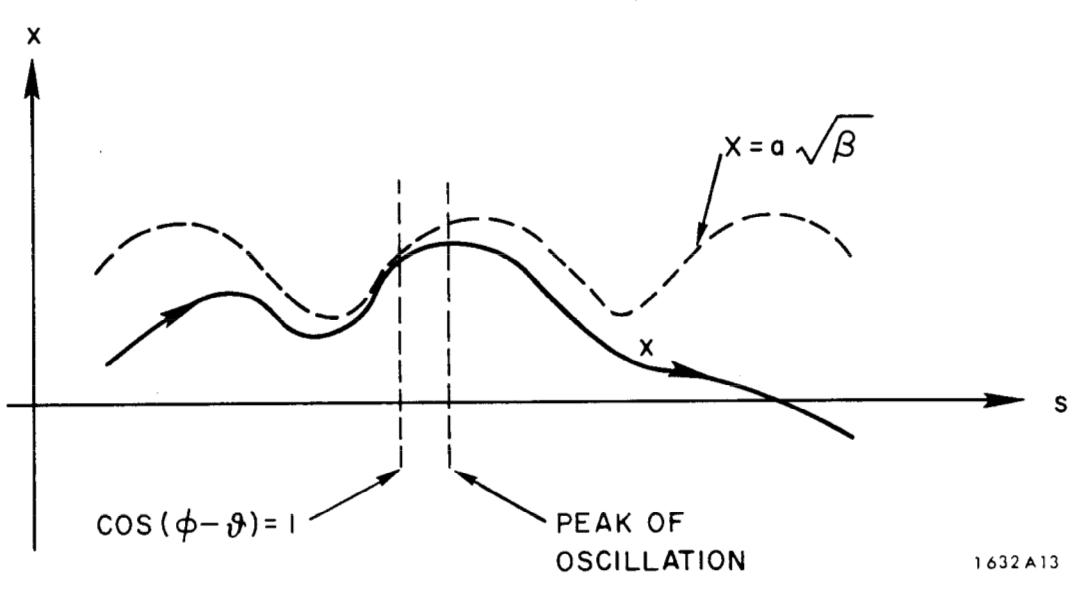
\includegraphics[width=0.8\linewidth]{./Figuras/fig13.jpeg}
	\caption{O máximo de um ciclo particular de uma oscilação betatron. Retirado de \cite{sands1970physics}.}
	\label{fig:fig13}
\end{figure}
	
Em uma oscilação harmônica clássica, a amplitude é uma invariante do movimento. Seu quadrado é proporcional à energia da oscilação, e pode ser expresso como uma função quadrática da posição e velocidade instantâneas. O invariante correspondente do oscilador pseudo-harmônico é a constante $a$, e esta pode ser obtida em termos de $x$ e $x'$ pela equação
	
\begin{align}
	a^2 = \frac{x^2}{\beta} + \beta\left[x'-\frac{\beta'}{2\beta}x\right]^2\label{eq:2.56}
\end{align}
	
\begin{proof}
	Pela equação \eqref{eq:2.43},
	\begin{align*}
        x &= a\sqrt{\beta}\ cos\{\varphi-\upsilon\}\\
        \frac{x}{a\sqrt{\beta}} &= cos(\varphi-\upsilon)\\
        \left(\frac{x}{a\sqrt{\beta}}\right)^2 &= cos^2(\varphi-\upsilon)\\
        \frac{x^2}{a^2\beta} &= cos^2(\varphi-\upsilon)
	\end{align*}
	
	Já pela equação \eqref{eq:2.52},
	\begin{align*}
        x' &= - \frac{a}{\sqrt{\beta}}sen(\varphi-\upsilon)+\frac{\beta'}{2\beta}x\\
        x' - \frac{\beta'}{2\beta}x&= - \frac{a}{\sqrt{\beta}}sen(\varphi-\upsilon)\\
        \frac{\sqrt{\beta}}{a}\left[x' - \frac{\beta'}{2\beta}x\right]&= -sen(\varphi-\upsilon)\\
        \left(\frac{\sqrt{\beta}}{a}\left[x' - \frac{\beta'}{2\beta}x\right]\right)^2&= sen^2(\varphi-\upsilon)\\
        \frac{\beta}{a^2}\left[x' - \frac{\beta'}{2\beta}x\right]^2&= sen^2(\varphi-\upsilon)
	\end{align*}
	
	Pela relação trigonométrica $sen^2(x)+cos^2(x)=1$,
	\begin{align*}
        sen^2(\varphi-\upsilon)+cos^2(\varphi-\upsilon)&=1\\
        \frac{\beta}{a^2}\left[x' - \frac{\beta'}{2\beta}x\right]^2 + \frac{x^2}{a^2\beta} &= 1\\
        \frac{1}{a^2}\left(\beta\left[x' - \frac{\beta'}{2\beta}x\right]^2 + \frac{x^2}{\beta}\right) &= 1\\
        \beta\left[x' - \frac{\beta'}{2\beta}x\right]^2 + \frac{x^2}{\beta} &= a^2
	\end{align*}
	c.q.d.
\end{proof}
	
Se os valores de $x$ e $x'$ são conhecidos em alguma coordenada, supõe-se $s_1$, então a constante $a$ pode ser obtida e todos os valores subsequentes de $x$ e $x'$ podem ser expressos por
	
\begin{align}
	x = \frac{1}{\sqrt{\beta_1}}\left[x_1^2+\left(\beta_1x'_1-\frac{x_1\beta'_1}{2}\right)^2\right]^\frac{1}{2}\sqrt{\beta}\ cos(\varphi-\upsilon)\label{eq:2.57}
\end{align}
	
\begin{proof}
	Pela equação \eqref{eq:2.56},
	\begin{align*}
        a^2 &= \frac{x^2}{\beta} + \beta\left[x'-\frac{\beta'}{2\beta}x\right]^2\\
        	&= \frac{1}{\beta}\left(x^2 + \beta^2\left[x'-\frac{\beta'}{2\beta}x\right]^2\right)\\
        	&= \frac{1}{\beta}\left(x^2 + \left[\beta x'-\frac{\beta'}{2}x\right]^2\right)\\
        \therefore a &= \left[\frac{1}{\beta}\left(x^2 + \left[\beta x'-\frac{\beta'}{2}x\right]^2\right)\right]^\frac{1}{2}\\
        	&= \frac{1}{\sqrt{\beta}}\left(x^2 + \left[\beta x'-\frac{\beta'}{2}x\right]^2\right)^\frac{1}{2}
	\end{align*}
	
	Sejam $x(s_1)=x_1$, $x'(s_1)=x'_1$ e $\beta(s_1)=\beta_1$ os valores de $x$, $x'$ e $\beta$ conhecidos no ponto $s_1$, então $a$ pode ser determinado com estes valores:
	\begin{align*}
		a = \frac{1}{\sqrt{\beta_1}}\left(x_1^2 + \left[\beta_1 x_1'-\frac{\beta_1'}{2}x_1\right]^2\right)^\frac{1}{2}
	\end{align*}
	
	Substituindo o valor de $a$ na equação \eqref{eq:2.43},
	\begin{align*}
		x &= a\sqrt{\beta}\ cos\{\varphi-\upsilon\}\\
		  &= \frac{1}{\sqrt{\beta_1}}\left[x_1^2+\left(\beta_1x'_1-\frac{x_1\beta'_1}{2}\right)^2\right]^\frac{1}{2}\sqrt{\beta}\ cos(\varphi-\upsilon)
	\end{align*}
	c.q.d.
\end{proof}
	
A constante de fase $\upsilon$ também precisa ser determinada de $x$ e $x'$, e esta pode ser obtida pela equação
	
\begin{align}
	tg(\varphi_1 - \upsilon) = -\frac{\beta_1 x'_1}{x_1}+\frac{\beta'_1}{2}
\end{align}
onde $\varphi_1 = \varphi(s_1)$.
	
\begin{proof}
	Já foi deduzido anteriormente que
	\begin{align*}
        sen(\varphi-\upsilon) &= -\frac{\sqrt{\beta}}{a}\left[x' - \frac{\beta'}{2\beta}x\right]\\
        cos(\varphi-\upsilon) &= \frac{x}{a\sqrt{\beta}}
	\end{align*}
	
	Para obter $tg(\varphi-\upsilon)$, basta
	\begin{align*}
		tg(\varphi-\upsilon) &= \frac{sen(\varphi-\upsilon)}{cos(\varphi-\upsilon)}\\
							 &= \frac{-\frac{\sqrt{\beta}}{a}\left[x' - \frac{\beta'}{2\beta}x\right]}{\frac{x}{a\sqrt{\beta}}}\\
							 &= -\frac{\sqrt{\beta}}{a}\left[x' - \frac{\beta'}{2\beta}x\right] \frac{a\sqrt{\beta}}{x}\\
							 &= \frac{\beta}{x}\left[-x' + \frac{\beta'}{2\beta}x\right]\\
							 &= -\frac{\beta x'}{x} + \frac{\beta'}{2}\\
		\therefore tg(\varphi_1-\upsilon) &= -\frac{\beta_1  x_1'}{x_1} + \frac{\beta_1'}{2}
	\end{align*}
	
	Isolando $\upsilon$, pode-se obtê-lo diretamente pela relação
	\begin{align*}
		tg(\varphi_1-\upsilon) &= -\frac{\beta_1  x_1'}{x_1} + \frac{\beta_1'}{2}\\
		cotg(tg(\varphi_1-\upsilon)) &= cotg\left(-\frac{\beta_1  x_1'}{x_1} + \frac{\beta_1'}{2}\right)\\
		\varphi_1-\upsilon &= cotg\left(-\frac{\beta_1  x_1'}{x_1} + \frac{\beta_1'}{2}\right)\\
		\upsilon &= \varphi_1 - cotg\left(-\frac{\beta_1  x_1'}{x_1} + \frac{\beta_1'}{2}\right)
	\end{align*}
\end{proof}
	
Para obter o valor máximo $X(s)$ que pode ser alcançado em qualquer $s$ em qualquer revolução subsequente, basta substituir $cos(\varphi-\upsilon)=1$ na equação \eqref{eq:2.57}:
	
\begin{align}
	X(s) = \frac{1}{\sqrt{\beta_1}}\left[x_1^2+\left(\beta_1x'_1-\frac{x_1\beta'_1}{2}\right)^2\right]^\frac{1}{2}\sqrt{\beta(s)}
\end{align}
	
Note que $X(s)$ independe de $\upsilon$.
	
Geralmente, é esperado que as amplitudes resultantes de distúrbios na trajetória serão menores quanto menor for $\beta$. De fato, pode-se considerar que $\frac{1}{\beta}$ é uma medida da "força" da focalização lateral, e que pequenos valores de $\beta$ são normalmente desejáveis. 
    \subsection{Sintonias}
	\subsection{Descrição aproximada das oscilações betatron}
Para diversos propósitos, é conveniente -- e suficiente -- aproximar o movimento betatron por uma oscilação harmônica simples. Considera-se a oscilação
\begin{align}
	x = A\ cos(s/ \lambdabar - \upsilon)\label{eq:2.66}
\end{align}
onde $\lambdabar$ é constante (o comprimento de onda reduzido). Uma oscilação completa é realizada quando $s$ avança por um comprimento de onda $2\pi \lambdabar$. É claramente conveniente pensar na oscilação pseudo-harmônica da equação \eqref{eq:2.43} como apenas uma onda senoidal com um comprimento de onda localmente variável -- se a variação de amplitude for ignorada. E, com tanto que $\beta$ não varie tão abruptamente, pode-se esperar que esta é uma aproximação razoável para o movimento real se a equação \eqref{eq:2.66} for utilizada com um $\lambdabar$ escolhido apropriadamente. Supõe-se que o número $\beta_n$ seja definido de forma a ser uma constante que dará o mesmo avanço de fase em uma revolução que a real função $\beta$. Isto é, $\beta_n$ é definido por
\begin{align}
	\int\limits_{0}^{L} \frac{ds}{\beta} = \frac{L}{\beta_n}\label{eq:2.67}
\end{align}
e é chamado de valor típico de $\beta$. Então, a oscilação
\begin{align}
	x = A\ cos(s/\beta_n + \upsilon)\label{eq:2.68}
\end{align}
irá -- com $A=a\sqrt{\beta_n}$ -- estar de acordo com a trajetória real pelo menos uma vez a cada revolução; e, em particular, irá estar, na média, em fase com a oscilação real. Na \autoref{fig:fig15} estão representadas uma das trajetórias da \autoref{fig:fig12} junto com sua aproximação obetida pela equação \eqref{eq:2.66}.

\begin{figure}[!htb]
	\centering
	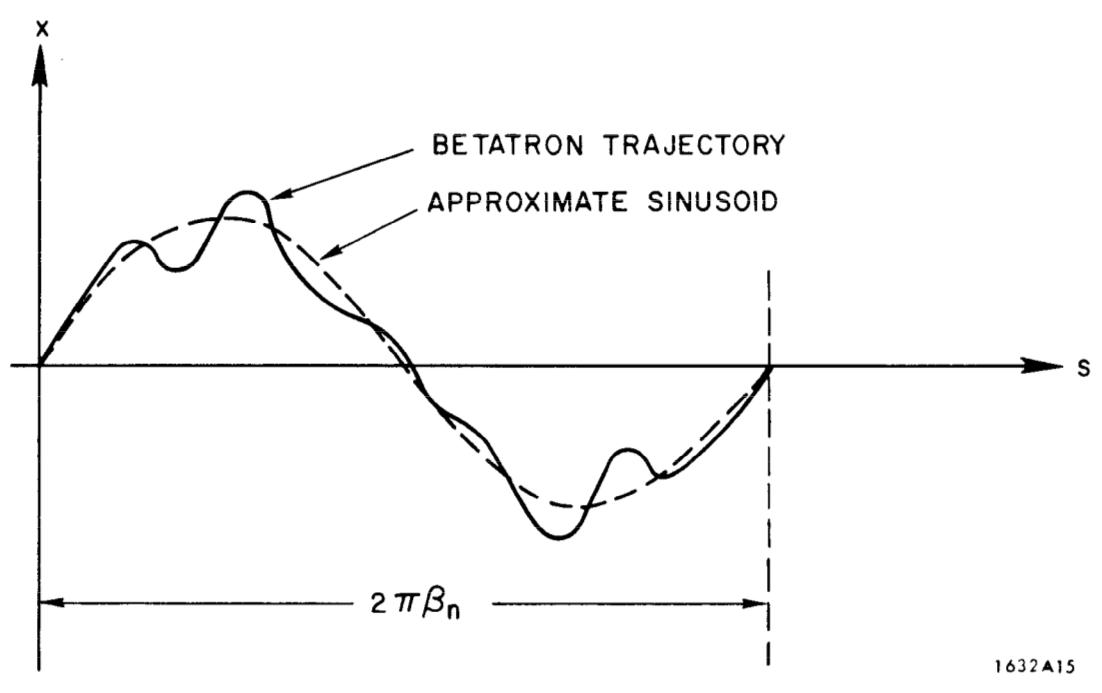
\includegraphics[width=0.7\linewidth]{./Figuras/fig15.jpeg}
	\caption{Aproximação da trajetória betatron.  ------ trajetória betatron; -- -- --  aproximação senoidal. Retirado de \cite{sands1970physics}.}
	\label{fig:fig15}
\end{figure}

É conveniente lembrar que, pela equação \eqref{eq:2.67}, $\frac{1}{\beta_n}$ é apenas a média de $\frac{1}{\beta}$ ao redor do anel:
\begin{align}
	\frac{1}{\beta_n} = \left \langle \frac{1}{\beta} \right \rangle
\end{align}

Pela definição de $\nu$ (equação \eqref{eq:2.60}), tem-se
\begin{align}
	\frac{L}{\beta_n} = 2\pi \nu
\end{align}

O raio efetivo de curvatura da órbita é dado por
\begin{align}
	R = \frac{L}{2\pi}
\end{align}
então pode-se também definir como
\begin{align}
	\beta_n = \frac{R}{\nu}
\end{align}

Note que $\beta_n$ não é igual à média de $\beta$, apesar de que também não é muito diferente se as ondulações de $\beta$ não forem muito grandes.

\begin{proof}
	Pela definição de $\nu$ e $\beta_n$ dadas respectivamente pelas equações \eqref{eq:2.60} e \eqref{eq:2.67},
	\begin{align*}
		\nu &= \frac{1}{2\pi} \int\limits_{0}^{L}\frac{ds}{\beta}\\
			&= \frac{1}{2\pi} \frac{L}{\beta_n}\\
		\therefore \frac{L}{\beta_n} &= 2\pi \nu
	\end{align*}
	
	Mas $R = L/2\pi$. Então,
	\begin{align*}
		\frac{L}{\beta_n} &= 2\pi \nu\\
		\therefore \beta_n &= \frac{L}{2\pi \nu}\\
						   &= \frac{R}{\nu}
	\end{align*}
\end{proof}

A variação de tempo da trajetória aproximada da equação \eqref{eq:2.68} é descrita como
\begin{align}
	x = A\ cos(\nu \omega_r t - \upsilon)
\end{align}
com $\omega_r = c/R$.

\begin{proof}
	Pela equação \eqref{eq:2.68}, $x = A\ cos(s/\beta_n - \upsilon)$. Agora, considerando como 0 a coordenada $s$ de referência, pela equação \eqref{eq:2.48}:
	\begin{align*}
		x &= A\ cos(s/\beta_n - \upsilon)\\
		  &= A\ cos(ct/\beta_n - \upsilon)\\
		  &= A\ cos(\nu c t/R - \upsilon)
	\end{align*}
	
	Definindo $\omega_r = c/R$, tem-se
	\begin{align*}
		x &= A\ cos(\nu \omega_r t - \upsilon)
	\end{align*}
	c.q.d.
\end{proof}

A frequência angular $\nu \omega_r$ é chamada de frequência betatron e será denominada por $\omega_\beta$. Note que, quando a trajetória aproximada é observada em um ponto fixo do anel, sua variação de tempo é indistinguível da trajetória real -- basta comparar com a equação \eqref{eq:2.64}.

A aproximação realizada nesta Seção não é adequada para vários cálculos dos efeitos do anel, mas de fato providencia a única abordagem rastreável para a análise de alguns dos efeitos coletivos que envolvem um número grande de elétrons armazenados.
	\subsection{Natureza da função beta}\label{sec:2.9}
Qual é a forma desejada de $\beta(s)$? Já foi visto que, pelo menos em alguns aspectos, pequenos valores de $\beta$ (focalização forte) são desejados -- tal que $\beta$ seja razoavelmente uniforme. Infelizmente, pequenos valores de $\beta$ só podem ser obtidos alternando o gradiente de focalização, o que tende a gerar oscilações razoavelmente grandes em $\beta$. Além disso, pequenos valores de $\beta$ implicam em grandes valores de $\nu$, o que pode gerar maiores dificuldades ao se lidar com as ressonâncias. Normalmente, $\beta$ tem um valor típico entre $1/2$ e $1/6$ do raio de curvatura $R$, não tendo, assim, oscilações muito extremas.

A função betatron é definida pela função singular, contínua a qual sua raiz quadrada satisfaz
\begin{align}
	\zeta'' = -K(s)\zeta + \frac{1}{\zeta^3}\label{eq:2.74}
\end{align}
onde $K(s)$ é a função de focalização. Tipicamente, os anéis modernos são feitos de vários segmentos nos quais a função $K(s)$ é constante, podendo ser nula, positiva ou negativa.

A imposição de que $\zeta(s)$ tem que ser periódica, juntamente com o termo não linear $1/\zeta^3$, gera uma especificação única -- incluindo a escala. A função $\zeta(s)$ é a função própria da equação \eqref{eq:2.74} e, por causa da não-linearidade, não existe uma normalização arbitrária da amplitude.

Fazendo uma análise dimensional, espera-se que $\zeta$ tenha uma dimensão $|K|^\frac{-1}{4}$, ou que $\beta$ tenha uma dimensão $|K|^\frac{-1}{2}$. (Relembrando que $1/\beta$ é como se fosse a frequência da oscilação, então é esperado que esta esteja de acordo com a raiz da constante da força restauradora). Para uma dada geometria do campo, esta lei de escala é grosseiramente verdadeira. Ela é estritamente verdadeira se a escala do comprimento da geometria de focalização é escalada em $|K|^\frac{-1}{2}$, o que geralmente é válido em campos guia bem projetados.

Em uma região de $s$ em que $K(s)$ é constante, a equação \eqref{eq:2.74} tem a forma da equação de movimento de uma partícula sob o efeito de uma força restauradora $-K\zeta$ e uma força repulsiva $1/\zeta^3$. Ou, da mesma forma, uma partícula que se move com uma energia potencial proporcional a
\begin{align}
	K\zeta^2 + \frac{1}{\zeta^2}
\end{align}
(O segundo termo é como se fosse uma barreira centrífuga!). O formato do potencial efetivo é mostrado na \autoref{fig:fig16} para os três casos de $K$.

\begin{figure}[!htb]
	\centering
	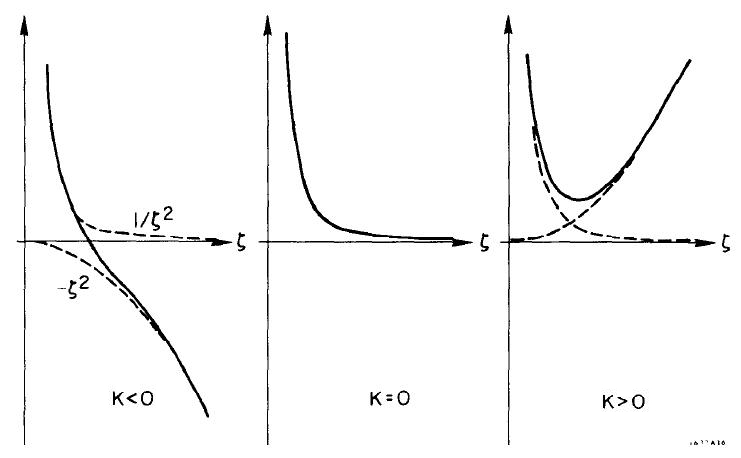
\includegraphics[width=0.9\linewidth]{./Figuras/fig16.jpeg}
	\caption{Funções potenciais efetivas para $\zeta$. Retirado de \cite{sands1970physics}.}
	\label{fig:fig16}
\end{figure}

Em qualquer região onde $K\leq 0$, a aceleração em $\zeta$ (o desvio da partícula de referência) é sempre positiva; e $\zeta$ é direcionado sempre para valores maiores -- ou, claro, dar a volta caso sua velocidade inicial seja na direção da origem de $\zeta$. Para $K$ negativo, a força direcional é, em grandes valores de $\zeta$, proporcional ao tamanho de $K$. Por outro lado, em qualquer região onde $K>0$, haverá um potencial estável e, quando $\zeta$ assume grandes valores, sempre há uma força direcionando $\zeta$ para a origem.

Também é qualitativamente aparente que possa existir soluções estáveis onde $\zeta(s)$ entra numa região onde $K<0$ movendo-se em direção à origem e muda de sentido devido à força de repulsão apenas para ser mandado na direção da origem novamente pela força de atração numa região posterior onde $K>0$. Para um K periódico como o da \autoref{fig:fig17}(a), deve-se esperar uma solução para $\zeta(s)$ como a curva representada na parte (b). A solução exibe uma importante característica geral da função $\zeta$: seu máximo ocorre em seções focalizadoras -- onde $K>0$ -- e seu mínimo ocorre em seções desfocalizadoras ou neutras -- onde $K \leq 0$.

\begin{figure}[!htb]
	\centering
	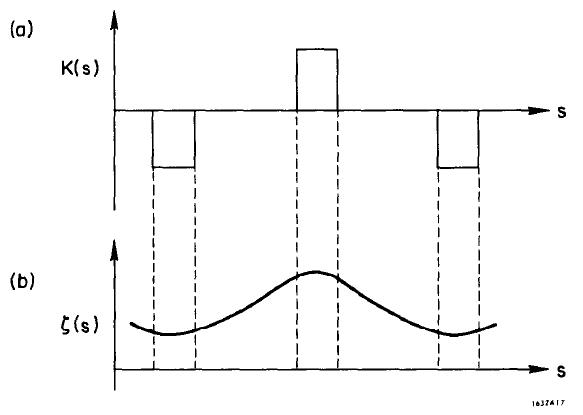
\includegraphics[width=0.7\linewidth]{./Figuras/fig17.jpeg}
	\caption{Forma da função $\zeta(s)$ com uma função de focalização $K(s)$ periódica. Retirado de \cite{sands1970physics}.}
	\label{fig:fig17}
\end{figure}

Também é evidente que para um determinado espaçamento com diferentes valores de $K$, se a magnitude de $K$ aumenta, a amplitude das oscilações irá crescer rapidamente. Menos evidente é o fato de que, conforme a escala de $K$ aumenta, chegará num ponto em que uma solução estável -- isto é, periódica -- para $\zeta(s)$ não existirá mais. Então a força de focalização (magnitude de $K$) e o espaçamento entre os elementos deve ser ajustado em conjunto, gerando a estrutura óptica do anel -- mais conhecida como \textit{lattice}, uma palavra para indicar a geometria dos segmentos.

Pode ocorrer o questionamento "Por que não apenas ter valores negativos de $K$ em todo $s$? Claramente a estabilidade de $\zeta$ é garantida". Isto não é possível pois quando $K$ é negativo em $x$, ele é automaticamente positivo em $z$, e vice-versa. Desta forma, fica claro que é necessário alternar o gradiente de focalização.

Também deve estar evidente que as oscilações de $\zeta(s)$ -- e, portanto, de $\beta(s)$ -- estarão fora de fase nas duas coordenadas transversais: $x$ e $z$. Quando $\zeta)x$ estiver em seu máximo, $\zeta_z$ estará em seu mínimo. Este comportamento é válido até nas estruturas mais complexas -- apesar de não ser totalmente verdade que $\zeta_x$ e $\zeta_z$ tem totalmente a mesma forma. 
%Na \autoref{fig:fig18} está um exemplo das funções $\zeta_x$ e $\zeta_z$.

%\begin{figure}[!htb]
%	\centering
%	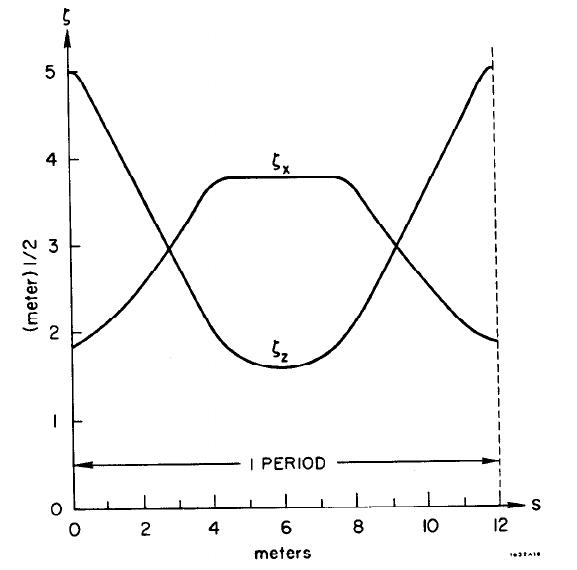
\includegraphics[width=0.7\linewidth]{./Figuras/fig18.jpeg}
%	\caption{Funções $\zeta_x$ e $\zeta_z$ de um campo guia. Retirado de \cite{sands1970physics}.}
%	\label{fig:fig18}
%\end{figure}

É intuitivo relacionar a função betatron $\beta(s)$ com a \textit{sine-like trajectory} definida na \autoref{sec:2.6}. A \textit{sine-like trajectory} $S(s,s_0)$ associada com a coordenada $s_0$ é a trajetória que começa em $s_0$ com deslocamento nulo e inclinação unitária. Esta pode ser expressa em termos da oscilação pseudo-harmônica dada pela equação \eqref{eq:2.43} substituindo $a=\sqrt{\beta(s_0)}$ e $\vartheta=\pi/2 + \varphi(s_0)$:
\begin{align}
	S(s,s_0) = \sqrt{\beta(s_0)\beta(s)}\ sen \left(\int\limits_{s_0}^{s} \frac{d\bar{s}}{\beta(\bar{s})}\right)
\end{align}
\begin{proof}
	Seja a trajetória dada pela equação \eqref{eq:2.43}:
	\begin{align*}
		x(s) = a\sqrt{\beta(s)}\ cos(\varphi(s)-\vartheta)
	\end{align*}
	com
	\begin{align*}
		\varphi(s) = \int\limits_{0}^{s} \frac{d\bar{s}}{\beta(\bar{s})}
	\end{align*}
	Substituindo $\vartheta=\pi/2 - \varphi(s_0)$:
	\begin{align*}
		x(s) &= a\sqrt{\beta(s)}\ cos(\varphi(s)-(\pi/2 + \varphi(s_0)))\\
			 &= a\sqrt{\beta(s)}\ sen(\varphi(s) - \varphi(s_0))
	\end{align*}
	Pela definição de $\varphi$,
	\begin{align*}
		x(s) &= a\sqrt{\beta(s)}\ sen\left(\int\limits_{0}^{s} \frac{d\bar{s}}{\beta(\bar{s})} - \int\limits_{0}^{s_0} \frac{d\bar{s}}{\beta(\bar{s})}\right)\\
			 &= a\sqrt{\beta(s)}\ sen\left(\int\limits_{s_0}^{s} \frac{d\bar{s}}{\beta(\bar{s})}\right)
	\end{align*}
	Substituindo $a=\sqrt{\beta(s_0)}$:
	\begin{align*}
		x(s) &= \sqrt{\beta(s_0)}\sqrt{\beta(s)}\ sen\left(\int\limits_{s_0}^{s} \frac{d\bar{s}}{\beta(\bar{s})}\right)\\
			 &= \sqrt{\beta(s_0)\beta(s)}\ sen\left(\int\limits_{s_0}^{s} \frac{d\bar{s}}{\beta(\bar{s})}\right)\\
		\therefore S(s,s_0) &= \sqrt{\beta(s_0)\beta(s)}\ sen\left(\int\limits_{s_0}^{s} \frac{d\bar{s}}{\beta(\bar{s})}\right)
	\end{align*}
	Checando,
	\begin{align*}
		S(s_0,s_0) &= \sqrt{\beta(s_0)\beta(s_0)}\ sen\left(\int\limits_{s_0}^{s_0} \frac{d\bar{s}}{\beta(\bar{s})}\right)\\
				   &= \beta(s_0)\ sen(0)\\
				   &= 0\\
		S(s,s_0)' &= \left(\sqrt{\beta(s_0)\beta(s)}\ sen\left(\int\limits_{s_0}^{s} \frac{d\bar{s}}{\beta(\bar{s})}\right)\right)'\\
				  &= \left(\sqrt{\beta(s_0)\beta(s)}\right)'\ sen\left(\int\limits_{s_0}^{s} \frac{d\bar{s}}{\beta(\bar{s})}\right) + \sqrt{\beta(s_0)\beta(s)}\ \left(sen\left(\int\limits_{s_0}^{s} \frac{d\bar{s}}{\beta(\bar{s})}\right)\right)'\\
				  &= \frac{1}{2}\frac{1}{\sqrt{\beta(s_0)\beta(s)}}(\beta(s_0)\beta(s))'\ sen\left(\int\limits_{s_0}^{s} \frac{d\bar{s}}{\beta(\bar{s})}\right) + \sqrt{\beta(s_0)\beta(s)}\ cos\left(\int\limits_{s_0}^{s} \frac{d\bar{s}}{\beta(\bar{s})}\right) \frac{1}{\beta(s)}\\
		S(s_0,s_0)' &= \frac{1}{2}\frac{1}{\sqrt{\beta(s_0)\beta(s_0)}}(\beta(s_0)\beta(s_0))'\ sen\left(\int\limits_{s_0}^{s_0} \frac{d\bar{s}}{\beta(\bar{s})}\right) + \sqrt{\beta(s_0)\beta(s_0)}\ cos\left(\int\limits_{s_0}^{s_0} \frac{d\bar{s}}{\beta(\bar{s})}\right) \frac{1}{\beta(s_0)}\\
					&= \frac{1}{2}\frac{1}{\beta(s_0)}(\beta(s_0)\beta(s_0))'\ sen(0) + \beta(s_0)\ cos(0) \frac{1}{\beta(s_0)}\\
					&= 0 + \beta(s_0)\frac{1}{\beta(s_0)}\\
					&= 1
	\end{align*}
	c.q.d.
\end{proof}

Agora, considere o que acontecerá se esta trajetória senoidal for seguida por uma volta completa -- ou seja, $s=s_0+L$. A integral fica, pela equação \eqref{eq:2.60}, apenas $2\pi\nu$. Devido à periodicidade da função betatron, $\beta(s_0+L) = \beta(s_0)$. Então,
\begin{align}
	S(s_0+L,s_0) = \beta(s_0)\ sen(2\pi\nu)
\end{align}
e, como $\nu$ independe de $s_0$, pode-se escrever também
\begin{align}
	\beta(s) = \frac{S(s+L,s)}{sen(2\pi\nu)}\label{eq:2.77}
\end{align}
Assim, a função betatron em $s$ é, a menos de uma constante, apenas o desvio após uma revolução da \textit{sine-like trajectory} começando em $s$. Veja a \autoref{fig:fig19}.

\begin{figure}[!htb]
	\centering
	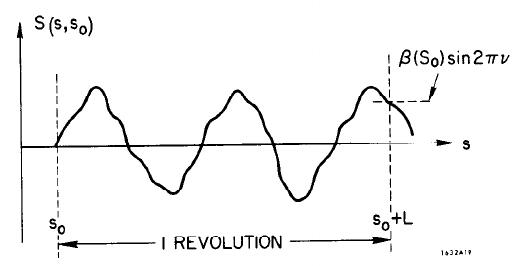
\includegraphics[width=0.8\linewidth]{./Figuras/fig19.jpeg}
	\caption{Relação entre $S(s,s_0)$ e $\beta(s_0)$. Retirado de \cite{sands1970physics}.}
	\label{fig:fig19}
\end{figure}

Pode-se obter uma outra prescrição para encontrar $\beta(s)$. Uma que precisa apenas do cálculo direto da \textit{sine-like trajectory} após uma revolução, começando em cada $s$.

O desvio obtido é proporcional a $\beta(s)$. Apenas resta determinar o fator de normalização $1/2\pi\nu$. Usando a definição de $\nu$ dada pela equação \eqref{eq:2.60}, juntamente com a equação \eqref{eq:2.77}, pode-se observar que a sintonia $\nu$ pode ser obtida como a solução da equação transcendental
\begin{align}
	\frac{2\pi\nu}{sen(2\pi\nu)} = \int\limits_{0}^{L} \frac{ds}{S(s+L,s)}
\end{align}
Então, conhecendo $S(s+L,s)$ para todo $s$, pode-se determinar $\beta(s)$ de forma única.

O cálculo de $S(s+L,s)$ pode ser efetuado por uma integração numérica da equação de movimento. Ou, para um campo guia uniforme, também pode ser obtido utilizando o método matricial descrito na \autoref{sec:2.5}. Relembrando a equação \eqref{eq:2.37}, a \textit{sine-like trajectory} de $s_0$ para $s_0+L$ é apenas o elemento da primeira linha e da primeira coluna da matriz de transferência $\boldsymbol{M}(s,s_0)$ para a máquina completa, começando em cada $s_0$.

Também pode-se mostrar que a sintonia $\nu$ pode ser obtida pelo traço da matriz para o anel todo:
\begin{align}
	cos(2\pi\nu) = \frac{1}{2} Tr \boldsymbol{M}(s+L,s) = \frac{1}{2}[C(s+L,s) + S'(s+l,s)]
\end{align}
onde $C$ é a \textit{cosine-like trajectory}. Então, se $C$ e $S'$ são calculados assim como $S$, $\nu$ pode ser determinada e a equação \eqref{eq:2.77} pode ser obtida diretamente.

Pode-se escrever a equação diferencial \eqref{eq:2.74} de $\zeta$ em termos de $\beta$:
\begin{align}
	\frac{1}{2}\beta\beta'' - \frac{1}{4}\beta'^2 + K(s)\beta^2 = 1\label{eq:2.80}
\end{align}

\begin{proof}
	Seja a equação diferencial $\zeta'' = -K(s)\zeta + \frac{1}{\zeta^3}$. Substituindo $\zeta = \sqrt{\beta}$,
	\begin{align*}
		\sqrt{\beta}'' &= -K\sqrt{\beta} + \frac{1}{\sqrt{\beta}^3}\\
		\left(\beta^\frac{1}{2}\right)'' &= -K\beta^\frac{1}{2} + \frac{1}{\beta^\frac{3}{2}}\\
		\left(\beta^\frac{1}{2}\right)''\beta^\frac{3}{2} &+ K\beta^\frac{1}{2} \beta^\frac{3}{2} = 1\\
		\left(\beta^\frac{1}{2}\right)''\beta^\frac{3}{2} &+ K\beta^2 = 1
	\end{align*}
	Derivando,
	\begin{align*}
		\left(\beta^\frac{1}{2}\right)''\beta^\frac{3}{2} + K\beta^2 &= 1\\
		\left(\frac{1}{2}\beta^\frac{-1}{2}\beta'\right)'\beta^\frac{3}{2} + K\beta^2 &= 1\\
		\left(\left(\beta^\frac{-1}{2}\right)'\beta' + \left(\beta^\frac{-1}{2}\right)\beta''\right)\frac{1}{2}\beta^\frac{3}{2} + K\beta^2 &= 1\\
		\left(\frac{-1}{2}\beta^\frac{-3}{2}\beta'\beta' + \beta^\frac{-1}{2}\beta''\right)\frac{1}{2}\beta^\frac{3}{2} + K\beta^2 &= 1\\
		\frac{-1}{4}\beta'^2 + \frac{1}{2}\beta\beta'' + K\beta^2 &= 1
	\end{align*}
	c.q.d.
\end{proof}

A partir da equação \eqref{eq:2.80}, podem-se fazer algumas observações. Primeiramente, em um trecho reto do anel (sem campo magnético), $K(s)=0$ e a solução da equação \eqref{eq:2.80} é
\begin{align}
	\beta = \beta_0\left[1+\frac{(s-s_0)^2}{\beta_0^2}\right]
\end{align}
onde $s_0$ e $\beta_0$ são constantes adequadas. Se $\beta$ tem um ponto de mínimo em um trecho reto, então $\beta_0$ e $s_0$ são os valores de $\beta$ e $s$ neste mínimo.

\begin{proof}
	A equação diferencial a ser resolvida é
	\begin{align*}
		\frac{1}{2}\beta\beta'' - \left(\frac{\beta'}{2}\right)^2
	\end{align*}
	Esta é uma equação diferencial ordinária não-linear de segunda ordem. Esta também é uma equação autônoma, ou seja, é uma equação que não contem explicitamente a variável independente -- neste caso, a coordenada $s$. Com isso, pode-se tratar a variável $\beta$ como variável independente da equação, e definir uma segunda variável $\alpha$ tal que
	\begin{align*}
		\alpha(\beta) = -\frac{\beta'}{2}
	\end{align*}
	Desta forma,
	\begin{align*}
		\beta' = -2\alpha(\beta)
		\therefore \beta'' = -2\frac{d\alpha}{d \beta}\beta' = -2\frac{d\alpha}{d \beta}(-2\alpha) = 4\alpha\frac{d\alpha}{d\beta}
	\end{align*}
	Substituindo na equação diferencial,
	\begin{align*}
		2\alpha\beta\frac{d\alpha}{d\beta} &= 1 + \alpha^2\\
		\therefore \frac{2\alpha}{1+\alpha^2}d\alpha &= \frac{1}{\beta}d\beta
	\end{align*}
	Integrando ambos os lados da equação:
	\begin{align*}
		\int \frac{2\alpha}{1+\alpha^2}d\alpha &= \int \frac{d\beta}{\beta}\\
		ln(1+\alpha^2) &= ln(\beta) + c_1\\
		ln(1+\alpha^2) - ln(\beta) &= c_1\\
		ln\left(\frac{1+\alpha^2}{\beta}\right) &= c_1
	\end{align*}
	sendo $c_1$ uma constante qualquer. Pela definição de logaritmo,
	\begin{align*}
		\frac{1+\alpha^2}{\beta} &= c_2
	\end{align*}
	sendo $c_2$ a constante dada por $e^{c_1}$. Derivando ambos os lados da expressão:
	\begin{align*}
		\frac{d}{d\beta}\left(\frac{1+\alpha^2}{\beta}\right) = 0
	\end{align*}
	Integrando esta equação diferencial de $\beta_0$ a $\beta$, tem-se
	\begin{align*}
		\frac{1+\alpha^2}{\beta} - \frac{1+\alpha_0^2}{\beta_0} = 0
	\end{align*}
	Definindo a constante $\gamma_0 = \frac{1+\alpha_0^2}{\beta_0}$, tem-se que
	\begin{align*}
		\frac{1+\alpha^2}{\beta} - \gamma_0 &= 0\\
		\frac{1+\alpha^2}{\beta} &= \gamma_0\\
		1+\alpha^2 &= \beta \gamma_0\\
		\therefore \alpha &= \sqrt{\beta\gamma_0 -1}
	\end{align*}
	Mas $\alpha = -\beta'/2$. Então,
	\begin{align*}
		-\frac{1}{2}\frac{d\beta}{ds} &= \sqrt{\beta\gamma_0 -1}\\
		\therefore -\frac{d\beta}{2\sqrt{\beta\gamma_0 -1}} &= ds
	\end{align*}
	Integrando ambos os lados da equação:
	\begin{align*}
		\int\limits_{\beta_0}^{\beta}-\frac{d\beta}{2\sqrt{\beta\gamma_0 -1}} &= \int\limits_{s_0}^{s}ds\\
		\left.\begin{matrix}
		-\frac{1}{\gamma_0}\sqrt{\beta\gamma_0-1}
		\end{matrix}\ \right|^\beta_{\beta_0} &= \left.\begin{matrix}
				s
				\end{matrix}\ \right|^s_{s_0}\\
		-\frac{1}{\gamma_0}\left(\sqrt{\beta\gamma_0-1}-\sqrt{\beta_0\gamma_0-1}\right) &= s-s_0\\
		\frac{1}{\gamma_0}\left(\sqrt{\beta_0\gamma_0-1}-\sqrt{\beta\gamma_0-1}\right) &= s-s_0\\
		\sqrt{\beta_0\gamma_0-1}-\sqrt{\beta\gamma_0-1} &= \gamma_0(s-s_0)
	\end{align*}
	Como foi definido anteriormente, $\gamma_0 = \frac{1+\alpha_0^2}{\beta_0}$. Logo,
	\begin{align*}
		\sqrt{1-\alpha_0^2-1}-\sqrt{\beta\gamma_0-1} &= \gamma_0(s-s_0)\\
		-\alpha_0-\sqrt{\beta\gamma_0-1} &= \gamma_0(s-s_0)\\
		-\sqrt{\beta\gamma_0-1} &= \alpha_0+\gamma_0(s-s_0)\\
	\end{align*}
	Elevando ambos os lados da equação ao quadrado:
	\begin{align*}
		\beta\gamma_0-1 &= [\alpha_0+\gamma_0(s-s_0)]^2\\
		\therefore \beta &= \frac{1}{\gamma_0}[1+(\alpha_0+\gamma_0(s-s_0))^2]
	\end{align*}
	No ponto de mínimo da função, $\beta'=0$ e, portanto, $\alpha=0$. Substituindo na solução obtida:
	\begin{align*}
		\beta &= \beta_0\left[1+\frac{1}{\beta_0^2}(s-s_0)^2\right]
	\end{align*}
	c.q.d.
\end{proof}

A forma desta solução é ilustrada na \autoref{fig:fig20}. Note que o coeficiente do termo quadrático é o inverso do valor de $\beta$ no seu ponto mínimo -- quanto menor for $\beta_0$. mais rápido é o aumento de $\beta$ com o aumento da distância do ponto de mínimo.


Finalmente, observe que, em um segmento que $K$ é grande e $\beta'$ pequeno, a equação \eqref{eq:2.80} pode ser aproximada por
\begin{align}
	\beta'' = -2K\beta
\end{align}
Assim, $\beta$ é uma senoide ou uma exponencial dependendo do sinal de $K$.

\begin{figure}[!htb]
	\centering
	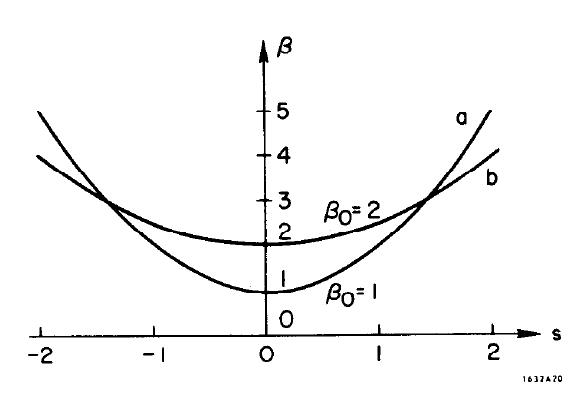
\includegraphics[width=0.7\linewidth]{./Figuras/fig20.jpeg}
	\caption{Variação de $\beta$ próximo do mínimo o qual ocorre em um longo trecho reto (sem campo magnético). Retirado de \cite{sands1970physics}.}
	\label{fig:fig20}
\end{figure}
	\subsection{Perturbação de órbita fechada}\label{sec:2.10}
Até o presente momento, foram consideradas as trajetórias de um elétron em um campo guia pré-definido. Agora, deseja-se considerar a seguinte pergunta: suponha que toda a análise sobre a trajetória dos elétrons foi feita acerca de um campo guia pré-definido; como as trajetórias irão variar se existirem pequenos erros no campo com relação ao campo pré-definido? Considerando a aproximação linear realizada até aqui, o campo guia pré-definido -- ou nominal -- é especificado pelo seu valor na órbita ideal e sua derivada radial. Além disso, assume-se que o campo na órbita ideal é vertical em todo o anel. E se o campo magnético vertical na órbita ideal diferir do seu valor nominal, ou se existirem pequenas componentes horizontais de campo, as acelerações laterais serão diferentes das especificações necessárias para manter o elétron na órbita ideal. Os desvios do campo na órbita ideal serão chamam-se erros de campo, enquanto mudanças no campo que fazem com que as funções de focalização $K_x$ e $K_z$ tenham valores diferentes de seus valores nominais chamam-se erros de gradiente.

Quando existem erros de campo, a órbita ideal deixa de ser uma trajetória possível. Se os erros são pequenos, no entanto, irá existir uma outra órbita fechada a qual é uma trajetória possível a um elétron com energia nominal. Esta trajetória é chamada de órbita fechada. Esta trajetória irá executar as oscilações betatron relativas à órbita fechada. E a forma das oscilações betatron será determinada pelas novas funções de focalização. Isto é, mantendo $x$ como sendo a representação do desvio radial da órbita ideal, este pode ser descrito como
\begin{align}
	x = x_c + x_\beta\label{eq:2.83}
\end{align}
onde $x_c$ é o desvio da órbita fechada com relação à órbita ideal, e $x_\beta$ é a oscilação betatron com relação à órbita fechada.

Se os desvios da órbita fechada com relação à órbita ideal são pequenos, então as oscilações betatron são as mesmas, tanto com relação à órbita ideal quanto com relação à órbita fechada -- assumindo uma variação linear do campo. Desta forma, pode-se considerar separadamente a distorção da órbita fechada causada pelos erros de campo e os distúrbios nas oscilações betatron causados pelos erros de gradiente. Seguindo esta ideia, a equação \eqref{eq:2.83} pode ser interpretada como uma superposição da distorção da órbita fechada $x_c$ e a oscilação betatron $x_\beta$ calculada com relação à órbita ideal pelos métodos já estudados.

Analisando primeiramente os erros de campo. Suponha que os efeitos dos erros de campo existentes apenas em pequenos intervalos $\Delta s$ analisados a partir de $s=0$ comecem a ser considerados. Passando por $\Delta s$, o desvio $x$ não se altera, mas a inclinação $x'$ é alterada pela quantidade
\begin{align}
	\Delta x' = -\frac{ec\ \delta B}{E_0}\Delta s
\end{align}
onde $\delta B$ é o desvio do campo magnético com relação ao seu valor nominal.

\begin{proof}
	Fazendo um raciocínio bem informal, já foi visto que
	\begin{align*}
		d\theta = -\frac{ecB}{E}d\ell
	\end{align*}
	Considerando $d\ell$ pequeno, pode-se aproximar que $dx = d\ell$. Assim,
	\begin{align*}
		d\theta = -\frac{ecB}{E}ds
	\end{align*}
	Analisando apenas para uma pequena modificação no campo magnético, para um elétron com energia nominal:
	\begin{align*}
		d\theta = -\frac{ec\ \delta B}{E_0}ds
	\end{align*}
	Analisando para um intervalo $\Delta s$,
	\begin{align*}
		\Delta\theta = -\frac{ecB}{E}\Delta s
	\end{align*}
	Mas $\Delta \theta$ é a variação da inclinação $x'$, logo
	\begin{align*}
		\Delta x' = -\frac{ecB}{E}\Delta s
	\end{align*}
	Uma formulação mais rigorosa pode ser obtida analisando a força de Lorentz.
\end{proof}

Para o movimento vertical, pode-se obter uma equação da mesma forma se $\delta B$ for definido como o campo radial total na órbita ideal (com uma escolha adequada de sinal). Mantendo a definição da equação \eqref{eq:2.3}, tem-se que $-ec\ \delta B/E_0 = -\delta G$, considerando as coordenadas transversais $x$ e $z$. Para facilitar a análise, será considerada apenas uma coordenada $x$ genérica, lembrando que os resultados obtidos valem tanto para o movimento radial quanto para o vertical. Desta forma, pode-se reescrever a equação anterior como sendo
\begin{align}
	\Delta x' = -\delta G \Delta s\label{eq:2.84}
\end{align}

O erro de campo adiciona à relação $x'' = \Delta x'/ \Delta s$ o termo $-\delta G$; e é, portanto, equivalente a adicionar uma força direcional $\delta G(s)$ à equação de movimento. Pode-se obter a equação completa para $x_c$ adicionando esta nova força à equação diferencial de costume, equação \eqref{eq:2.31}:
\begin{align}
	x'' = -K(s)x - \delta G(s)\label{eq:2.85}
\end{align}
O desvio $x_c$ da órbita fechada é a solução desta equação singular.

Pode-se fazer uma estimativa do efeito de um erro de campo localizado em $s=0$ usando a forma harmônica aproximada do movimento betatron descrita na \autoref{sec:2.8}. Pense em um elétron viajando ao longo da órbita ideal -- de forma que a inclinação $x'$ seja nula. Quando este elétron chegar em $s=0$, sua inclinação será subitamente alterada para $\Delta x'$. Veja a \autoref{fig:fig21}. 

\begin{figure}[!htb]
	\centering
	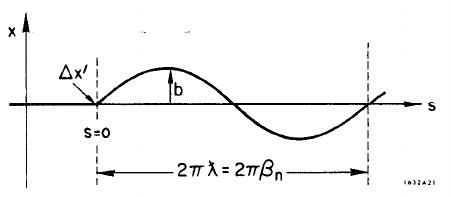
\includegraphics[width=0.7\linewidth]{./Figuras/fig21.jpeg}
	\caption{Efeito de um erro de campo localizado. Retirado de \cite{sands1970physics}.}
	\label{fig:fig21}
\end{figure}
Depois de $s=0$ não há erro de campo (para uma volta completa) então o elétron começa a oscilar em torno da órbita ideal com amplitude
\begin{align}
	b = \lambdabar \Delta x' = \beta_n \Delta x' = -\beta_n\ \delta G \Delta s\label{eq:2.86}
\end{align}
É esperado que o desvio da órbita fechada $x_c$ seja da mesma ordem de grandeza.

\begin{proof}
	Matematicamente, uma senoide com fase nula é descrita por
	\begin{align*}
		x(s) = b\ sen\left(\frac{2\pi s}{\lambda}\right)
	\end{align*}
	onde $b$ é a amplitude da oscilação e $\lambda$ é seu comprimento de onda. Desta forma,
	\begin{align*}
		x'(s) &= \frac{2\pi}{\lambda}b\ cos\left(\frac{2\pi s}{\lambda}\right)\\
		\therefore x'(0) & = \frac{2\pi}{\lambda}b\\
		\therefore b &= \frac{\lambda}{2\pi}x'(0)
	\end{align*}
	Já foi visto na \autoref{sec:2.8} que $\lambdabar = \lambda/2\pi$, então
	\begin{align*}
		b &= \lambdabar x'(0)
	\end{align*}
	Mas, considerando a análise que está sendo feita, $x'(0) = \Delta x'$. Logo,
	\begin{align*}
		b &= \lambdabar \Delta x'
	\end{align*}
	Também na \autoref{sec:2.8} mostrou-se que $\lambdabar = \beta_n$, então
	\begin{align*}
		b &= \beta_n \Delta x'\\
		  &= -\beta_n\ \delta G \Delta s
	\end{align*}
	c.q.d.
\end{proof}

Para fazer o cálculo de $x_c$ de forma apropriada, deve-se utilizar a oscilação pseudo-harmônica correta, e lembrar também que a órbita fechada é definida como a trajetória particular que fecha nela mesma após uma revolução. Em outras palavras, $x_c$ deve ser uma função singular em cada coordenada física $s$, ou seja, $x_c(s+L) = x_c(s)$. Em particular,
\begin{align}
	x_c(L) = x_c(0)\label{eq:2.87}
\end{align}
e, pela equação \eqref{eq:2.84},
\begin{align}
	x'_c(L) - \delta G \Delta s = x'_c(0)\label{eq:2.88}
\end{align}
Mas entre $s=0$ e $s=L$ não existem erros de campo, então $x_c$ é apenas uma oscilação livre entorno da órbita ideal. Veja a \autoref{fig:fig22}. Isto é, $x_c$ deve ser dado pela equação \eqref{eq:2.43}:
\begin{align}
	x_c(s) = a\sqrt{\beta(s)}cos(\varphi - \vartheta),\ s \neq 0,\label{eq:2.89}
\end{align}
com constantes arbitrárias $a$ e $\vartheta$ escolhidas de tal maneira que as equações \eqref{eq:2.87} e \eqref{eq:2.88} sejam satisfeitas.

\begin{figure}[!htb]
	\centering
	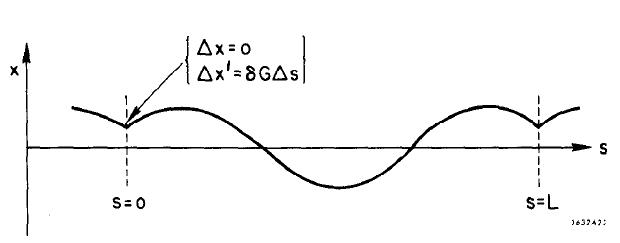
\includegraphics[width=0.7\linewidth]{./Figuras/fig22.jpeg}
	\caption{Órbita fechada para um erro de campo em $s=0$. Retirado de \cite{sands1970physics}.}
	\label{fig:fig22}
\end{figure}

Utilizando a equação \eqref{eq:2.52} para $x'_c(s)$ -- em todo o anel exceto em $s=0$ -- pode-se verificar que os valores apropriados para $a$ e $\vartheta$ são
\begin{align}
	a &= -\frac{\delta G\ \Delta s\ \sqrt{\beta(0)}}{2 sen(\pi \nu)}\\
	\vartheta &= \pi \nu
\end{align}

\begin{proof}
	Seja $x_c(L)$ dado pela equação \eqref{eq:2.89}:
	\begin{align*}
		x_c(L) = a\sqrt{\beta(L)}\ cos(\varphi(L)-\vartheta)
	\end{align*}
	Pela definição de $\varphi(s)$ e $\nu$,
	\begin{align*}
		x_c(L) = a\sqrt{\beta(L)}\ cos(2\pi\nu-\vartheta)
	\end{align*}
	Mas, a condição da equação \eqref{eq:2.87} deve ser satisfeita. Logo,
	\begin{align*}
		x_c(L) &= x_c(0)\\
		a\sqrt{\beta(L)}\ cos(2\pi\nu-\vartheta) &= a\sqrt{\beta(0)}\ cos(\varphi(0)-\vartheta)
	\end{align*}
	Novamente, pela definição de $\varphi(s)$,
	\begin{align*}
		a\sqrt{\beta(L)}\ cos(2\pi\nu-\vartheta) &= a\sqrt{\beta(0)}\ cos(-\vartheta)
	\end{align*}
	Pela periodicidade da função $\beta$,
	\begin{align*}
		a\sqrt{\beta(0)}\ cos(2\pi\nu-\vartheta) &= a\sqrt{\beta(0)}\ cos(-\vartheta)\\
		cos(2\pi\nu-\vartheta) &= cos(-\vartheta)
	\end{align*}
	Como cosseno é uma função par,
	\begin{align*}
		cos(2\pi\nu-\vartheta) &= cos(\vartheta)\\
		\therefore 2\pi\nu - \vartheta &= \vartheta\\
		\therefore \vartheta &= \pi\nu
	\end{align*}
	Agora, seja $x'_c(L)$ dado pela equação \eqref{eq:2.52}:
	\begin{align*}
		x'_c(L) &= -\frac{a}{\beta(L)}\ sen(\varphi(L)-\vartheta) + \frac{\beta'(L)}{2\beta(L)}x_c(L)\\
				&= -\frac{a}{\beta(L)}\ sen(2\pi\nu-\pi\nu) + \frac{\beta'(L)}{2\beta(L)}x_c(L)\\
				&= -\frac{a}{\beta(L)}\ sen(\pi\nu) + \frac{\beta'(L)}{2\beta(L)}x_c(L)
	\end{align*}
	A condição da equação \eqref{eq:2.88} impõe que
	\begin{align*}
		x'_c(L) - \delta G\ \Delta s &= x'_c(0)\\
		-\frac{a}{\beta(L)}\ sen(\pi\nu) + \frac{\beta'(L)}{2\beta(L)}x_c(L) - \delta G\ \Delta s &= -\frac{a}{\beta(0)}\ sen(\varphi(0)-\pi\nu) + \frac{\beta'(0)}{2\beta(0)}x_c(0)\\
		-\frac{a}{\beta(L)}\ sen(\pi\nu) + \frac{\beta'(L)}{2\beta(L)}x_c(L) - \delta G\ \Delta s &= -\frac{a}{\beta(0)}\ sen(0-\pi\nu) + \frac{\beta'(0)}{2\beta(0)}x_c(0)\\
		-\frac{a}{\beta(L)}\ sen(\pi\nu) + \frac{\beta'(L)}{2\beta(L)}x_c(L) - \delta G\ \Delta s &= -\frac{a}{\beta(0)}\ sen(-\pi\nu) + \frac{\beta'(0)}{2\beta(0)}x_c(0)
	\end{align*}
	Pela periodicidade da função $\beta(s)$ e a restrição imposta pela equação \eqref{eq:2.87},
	\begin{align*}
		-\frac{a}{\beta(0)}\ sen(\pi\nu) + \frac{\beta'(0)}{2\beta(0)}x_c(0) - \delta G\ \Delta s &= -\frac{a}{\beta(0)}\ sen(-\pi\nu) + \frac{\beta'(0)}{2\beta(0)}x_c(0)\\
		\therefore -\frac{a}{\beta(0)}\ sen(\pi\nu) - \delta G\ \Delta s &= -\frac{a}{\beta(0)}\ sen(-\pi\nu)
	\end{align*}
	Como seno é uma função ímpar,
	\begin{align*}
		-\frac{a}{\beta(0)}\ sen(\pi\nu) - \delta G\ \Delta s &= \frac{a}{\beta(0)}\ sen(\pi\nu)\\
		\therefore \frac{a}{\beta(0)}\ 2sen(\pi\nu) &= -\delta G\ \Delta s\\
		\therefore a = -\frac{\delta G\ \Delta s\ \sqrt{\beta(0)}}{2 sen(\pi \nu)}
	\end{align*}
	c.q.d.
\end{proof}

O desvio da órbita fechada é, portanto,
\begin{align}
	x_c(s) = -\frac{\delta G\ \Delta s\ \sqrt{\beta(0)}}{2 sen(\pi \nu)}\ \sqrt{\beta(s)}\ cos(\varphi(s)-\pi\nu)\label{eq:2.92}
\end{align}

A forma do invariante $a$ da amplitude mostra duas características interessantes da órbita fechada. Primeiramente, note que o desvio da órbita fechada é em todo o anel proporcional à "força" $\ \delta G \Delta s$ do erro de campo, e à raiz de $\beta(0)$, a magnitude da função betatron no local da perturbação. Agora entende-se porque $\beta(s)$ -- ou mais precisamente $\zeta(s) = \sqrt{\beta(s)}$ -- é uma medida da "sensibilidade" à distúrbios.

Segundo, note que o denominador de $a$ vai para zero, e $x_c$ se torna, portanto, muito grande sempre que a sintonia $\nu$ se aproxima de um inteiro. É este comportamento o qual foi referido anteriormente como "ressonância inteira", a qual deve ser evitada escolhendo o ponto de operação $(\nu_x,\nu_z)$ longe de números inteiros.

Note que o desvio da órbita fechada no local do erro de campo tem uma forma particularmente simples. Basta apenas analisar a equação \eqref{eq:2.92} considerando $s=0$, ou generalizar para um erro de campo localizado em uma coordenada arbitrária $s_1$, obtendo
\begin{align}
	x_c(s_1) = -\delta G\ \Delta s \frac{\beta(s_1)}{2 tg(\pi\nu)}
\end{align}
Agora o desvio é proporcional à primeira potência de $\beta$, mas a dependência da ressonância de $\nu$ ainda é evidente no termo da tangente. Note também que, exceto pelo denominador ressonante, o resultado confere com a estimativa dada pela equação \eqref{eq:2.86}.

A equação \eqref{eq:2.92} também pode ser generalizada para uma órbita fechada com erros de campo que seguem uma distribuição arbitrária ao longo do anel. Em cada coordenada $s$, os desvios da órbita fechada causados por erros em todas as outras coordenadas irão se somar. Para um erro em $\bar{s}$, deve-se substituir $s=0$ por $\bar{s}$ na equação \eqref{eq:2.92} -- e, ao mesmo tempo, substituir $\varphi(s)$ por $|\varphi(s) - \varphi\bar{s}|$. Assim, somando sobre todos os $\Delta \bar{s}$, tem-se 
\begin{align}
	x_c(s) = -\frac{\sqrt{\beta(s)}}{2sen(\pi\nu)}\int\limits_{0}^{L}\delta G(\bar{s})\sqrt{\beta(\bar{s})}cos(|\varphi(s)-\varphi(\bar{s})|-\pi\nu)d\bar{s}\label{eq:2.94}
\end{align}
Se o desvio de campo $\delta G(s)$ é conhecido, esta equação dará a forma da órbita fechada (considerando os valores nominais de $\beta(s)$ e $\nu$).

Se os desvios de campo são verdadeiros "erros" com uma distribuição estatística desconhecida, uma análise estatística mais complexa deve ser feita para chegar na estimativa estatística de $x_c$.

Como foi dito anteriormente, o desvio total da órbita ideal é dado pela soma de $x_c$ e a oscilação betatron. Na próxima análise, $x_c$ será ignorado -- lembrando sempre que este precisa ser adicionado quando pretende-se analisar o desvio total da trajetória com relação à órbita ideal.
	\subsection{Erros de gradiente de campo}
Agora, pode-se analisar os efeitos dos erros de gradiente nas oscilações betatron em torno da órbita ideal. estes "erros" são relativos aos desvios da função de focalização $K(s)$ do seu valor nominal em cada coordenada $s$. Pode-se escrever
\begin{align*}
	K(s)_{atual} = K(s)_{nominal} + k(s)
\end{align*}
onde assume-se que $k(s)$ é pequeno. O efeito do desvio $k(s)$ será mudar a função betatron do seu valor nominal $\beta(s)$ para um novo valor $\beta(s)+\Delta \beta(s)$. Desta forma, a sintonia também será alterada do seu valor nominal $\nu$ para um novo valor $\nu + \Delta \nu$. Geralmente, a mudança de sintonia $\Delta \nu$ é mais preocupante, uma vez que esta pequena mudança pode fazer com que o ponto de operação da máquina entra em uma ressonância.

Suponha que existe um erro de gradiente $k$ apenas em um pequeno intervalo $\Delta s$ em $s=0$. Então um elétron que passa em $s=0$ irá receber um \textit{kick} angular extra $\Delta x'$ proporcional ao seu desvio $x$. Isto é,
\begin{align}
	\Delta x' = -k\ \Delta s\ x\label{eq:2.96}
\end{align}

\begin{proof}
	Fazendo um raciocínio bem informal, sabe-se que a equação diferencial que descreve o movimento do elétron é
	\begin{align*}
		x'' = -K(s)x
	\end{align*}
	A derivada nada mais é que a variação de $x'$ em um intervalo $s$ pequeno, então $x'' = \Delta x'/\Delta s$. Logo,
	\begin{align*}
		\frac{\Delta x'}{\Delta s} &= -K(s)x\\
		\Delta x' &= -K(s)x \Delta s
	\end{align*}
	Analisando apenas a variação de $x'$ causada pela variação $k(s)$ da função de focalização, tem-se
	\begin{align*}
		\Delta x' &= -k\ \Delta s\ x
	\end{align*}
\end{proof}

Aproximando novamente a função betatron por uma simples oscilação harmônica, o que aconteceria se um elétron chegasse em $s=0$ no pico da oscilação? o movimento seria como a curva representada na \autoref{fig:fig23}.

\begin{figure}[!htb]
	\centering
	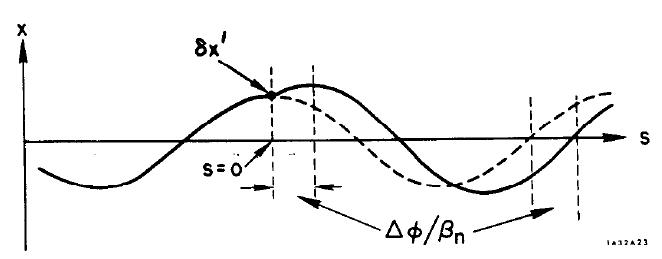
\includegraphics[width=0.7\linewidth]{./Figuras/fig23.jpeg}
	\caption{Efeito do gradiente de erro em $s=0$. Retirado de \cite{sands1970physics}.}
	\label{fig:fig23}
\end{figure}

Antes de chegar em $s=0$. o desvio era dado por
\begin{align}
	x = b\ cos(s/\beta_n)
\end{align}
e, depois de $s=0$, seguirá uma trajetória
\begin{align}
	x = (b+\Delta b)cos(s/\beta_n + \Delta \varphi)
\end{align}
onde
\begin{align}
	-\frac{b+\Delta b}{\beta_n}\ sen(\Delta \varphi) = \Delta x'
\end{align}

\begin{proof}
	Seja a solução da equação diferencial $x'' = -Kx$ dada por $x = a\ cos(\varphi-\vartheta)$. Para $K(s) = K(s)_{nominal}$ já foi visto que existe a solução aproximada $x = b\ cos(s/\beta_n)$. Quando o elétron passa em $s=0$, a equação diferencial deixa de ser $x'' = -K(s)_{nominal}\ x$ e passa a ser $x'' = -K(s)_{atual}\ x$ onde $K(s)_{atual} = K(s)_{nominal} + k(s)$. Logo, a equação diferencial é dada por $x'' = -(K(s)_{nominal} + k(s))x$. Esta mudança na função de focalização $K(s)$ acarretará numa mudança $\Delta \beta$ no valor da função betatron. Como tanto a amplitude quanto a fase de oscilação dependem de $\beta(s)$, ambas sofreram alterações, as quais foram denominadas $\Delta b$ e $\Delta \varphi$, respectivamente. Sendo assim, a solução desta nova equação diferencial pode ser escrita como
	\begin{align*}
		x = (b+\Delta b)\ cos(s/\beta_n + \Delta \varphi)
	\end{align*}
	Nota-se que o termo $\Delta \varphi$ não está multiplicado pela variável $s$ como o termo $1/\beta_n$. Isto porque a alteração na fase da oscilação ocorre somente no ponto $s=0$, diferentemente do avanço de fase descrito pelo termo $s/\beta_n$.
	
	Agora, derivando a expressão $x = b\ cos(s/\beta_n)$, tem-se
	\begin{align*}
		x' &= -b\ sen(s/\beta_n)\\
		\therefore x'(0) &= 0 = x'_i
	\end{align*}
	Derivando a expressão $x = (b+\Delta b)\ cos(s/\beta_n + \Delta \varphi)$, tem-se
	\begin{align*}
		x' = -\frac{b+\Delta b}{\beta_n}\ sen(s/\beta_n + \Delta \varphi)\\
		x'(0) = -\frac{b+\Delta b}{\beta_n}\ sen(\Delta \varphi) = x'_f
	\end{align*}
	Desta forma, a variação $\Delta x'$ da inclinação do movimento no ponto $s=0$ é
	\begin{align*}
		\Delta x' &= x'_f - x'_i\\
				  &= -\frac{b+\Delta b}{\beta_n}\ sen(\Delta \varphi) - 0\\
				  & = -\frac{b+\Delta b}{\beta_n}\ sen(\Delta \varphi)
	\end{align*}
	c.q.d.
\end{proof}

Para pequenos valores de $\Delta x'$, $\Delta \varphi$ é pequeno (ou seja, pode-se aproximar $sen(\varphi) = \varphi$) e $\Delta b$ é muito menor que $b$. Logo,
\begin{align}
	\Delta \varphi \approx -\frac{\beta_n\ \Delta x'}{b}
\end{align}
Utilizando a equação \eqref{eq:2.96} -- e lembrando que em $s=0$ o deslocamento é $b$ -- tem-se que
\begin{align*}
	\Delta \varphi = \beta_n\ k\ \Delta s
\end{align*}
O efeito do erro de gradiente é basicamente alterar a fase de oscilação por $\Delta \varphi$. Agora, lembre-se que $2\pi\nu$ é o avanço de fase total em uma revolução; então, grosseiramente falando, o erro de gradiente acarreta em
\begin{align}
	\Delta \nu \approx - \frac{\Delta \varphi}{2\pi} = -\frac{\beta_n\ k\ \Delta s}{2\pi}
\end{align}
O sinal negativo vem do fato de que o avanço total de fase é reduzido.

Este resultado é, na verdade, até duas vezes maior do que o normal. O motivo é que o cálculo de $\Delta \varphi$ foi feito no caso especial do elétron chegando em $s=0$ no pico da oscilação. Se o elétron chegar em $s=0$ com uma fase $\varphi_0$, a mudança de fase $\delta \varphi$ é reduzida por um fator $cos^2(\varphi_0)$. Como $\varphi_0$ assume vários valores ao longo de sucessivas voltas, pode-se esperar que a média de $\Delta \varphi$ seja reduzida pela média de $cos^2(\varphi_0)$, que é apenas $1/2$. Com esta correção, a estimativa de $\Delta \nu$ fica
\begin{align}
	\Delta \nu = -\frac{1}{4\pi}\beta(s)\ k\ \Delta s
\end{align}

Note que a mudança da sintonia é proporcional ao erro de gradiente em qualquer ponto e ao valor de $\beta$ neste ponto. Novamente, pode-se observar que a função $\beta$ é um indicador da sensibilidade do anel a imperfeições.

Se existe um erro de gradiente $k(s)$ distribuído ao longo do anel, a alteração total da sintonia é
\begin{align}
	\Delta \nu = -\frac{1}{4\pi} \int\limits_{0}^{L}\beta(s)k(s)ds\label{eq:2.104}
\end{align}

Foi dito anteriormente que é esperado que $\Delta \nu$ seja da dimensão de $\nu$, então grandes valores de $\nu$ devem ser evitados. Para checar este fato, lembre (da \autoref{sec:2.10}) que $\beta$ é esperado para ser escalado como $|K|^{-1/2}$. Sendo assim, $\nu$ deve ter a mesma dimensão que $|K|^{1/2}$. Da equação \eqref{eq:2.104}, $\Delta \nu$ deve ser da magnitude de $k\beta$, então $\Delta \nu/\nu$ deve ser da mesma dimensão que $k/K$. Para um dado tamanho relativo do erro de gradiente, a alteração da sintonia $\Delta \nu$ é proporcional a $\nu$. Mas o espaço entre as ressonâncias é independente de $\nu$, então grandes valores de $\nu$ implicam em uma máquina mais delicada.

Uma mudança em $\nu$ implica que deve ter ocorrido uma mudança em $\beta$, a qual ainda não ficou muito evidente nos cálculos realizados. Pode-se mostrar que
\begin{align}
	\Delta \beta(s) = \frac{\beta(s)}{2\ sen(2\pi\nu)}\int\limits_{0}^{L}k(\bar{s})\ \beta(\bar{s})\ cos\ 2\{|\varphi(s)-\varphi(\bar{s})|-\pi\nu\}d\bar{s}\label{eq:2.105}
\end{align}
onde, como já é conhecido,
\begin{align}
	\varphi(s) = \int\limits_{0}^{s}\frac{d\bar{s}}{\beta(\bar{s})}
\end{align}

Pode-se comparar este resultado com o que foi obtido na equação \eqref{eq:2.94} para as distorções de órbita fechada. A forma é similar, mas com duas diferenças importantes. Primeiro, enquanto $\beta^{1/2}$ aparece na integral para os desvios da órbita fechada, $\beta$ aparece na integral para $\Delta \beta$. Segundo, note que o argumento do termo senoidal no denominador é $2\pi\nu$ ao invés de $\pi\nu$. A "explosão" ressonante ocorre tanto nos valores inteiros quanto nos meio inteiros de $\nu$. O erro de gradiente introduz um novo grupo de ressonâncias no diagrama de operação de $\nu_x$ po $\nu_z$, as quais devem ser evitadas em um anel de armazenamento em operação.

A mudança de sintonia $\Delta \nu$ vem, claro, da mudança na função betatron. Da definição de $\nu$, pode-se escrever
\begin{align}
	2\pi\nu = \int\limits_{0}^{L}\frac{\Delta \beta(s)}{\beta^2(s)}ds
\end{align}
Uma integração em $s$ de $\Delta \beta(s)/\beta^2(s)$ utilizando a equação \eqref{eq:2.105} chega no mesmo resultado para $\Delta \nu$ obtido na equação \eqref{eq:2.104}.

Neste ponto, pode-se esperar um certo questionamento: por que $\Delta \beta$ tem uma explosão ressonante em valores meio inteiros de $\nu$ e a mudança de sintonia $\Delta \nu$ não? A razão para este fato é que a expressão derivada para $\Delta \nu$ é válida apenas para pequenas variações de $\beta$, o que não acontece em ressonâncias, nas quais $\beta$ diverge. Um cálculo mais preciso deve ser feito, mantendo os efeitos de segunda ordem causados pela perturbação $k$, para encontrar $\Delta \nu$ -- e, de fato, o próprio $\Delta \beta$ -- próximo a uma ressonância.
	\pagebreak
	
\section{Oscilações de Energia}
	\subsection{Órbitas fechadas}
Nas discussões anteriores, foram analisadas trajetórias em anéis de armazenamento de elétrons com energia nominal $E_0$ --  a qual é a energia projetada para uma dada configuração ótica. No entanto, nem todos os elétrons armazenados possuem esta energia ideal. No geral, a energia $E$ de um elétron armazenado irá diferir da energia nominal, oscilando em torno desta. Estas oscilações de energia -- comumente chamadas de ''oscilações síncronas'' -- são o objeto de estudo desta seção.

Primeiramente, é necessário entender o movimento destes elétrons cuja energia difere de uma pequena quantidade $\epsilon$ da energia nominal. Mantendo a condição da \autoref{sec:3.2} de que a órbita ideal se encontra no plano horizontal, desvios de energia irão, para termos de primeira ordem, afetar apenas o movimento radial. O desvio vertical irá ser descrito apenas pelas oscilações betatron descritas na \autoref{part2}, e não serão consideradas nesta análise. Da \autoref{sec:2.6}, foi conveniente deixar que o símbolo $x$ representasse tanto $x_\beta$ quando $z_\beta$, os desvios laterais associados às oscilações betatron. A partir de agora, $x$ volta a representar o desvio horizontal total da trajetória com relação à órbita ideal.

Foi mostrado na \autoref{sec:2.5} que em um campo guia ideal o movimento radial de um elétron com um desvio de energia $\epsilon$ pode ser descrito pela soma de duas partes:
\begin{align}
	x = x_\beta + x_\epsilon
\end{align}
onde $x_\beta$ é o desvio causado pelas oscilações betatron e $x_\epsilon$ o desvio que depende apenas da energia do elétron. Acrescentando os resultados obtidos na \autoref{sec:2.11}, deve-se incluir o termo referente à distorção da órbita fechada devido às imperfeições magnéticas e escrever
\begin{align}
	x = x_\beta + x_\epsilon + x_c
\end{align}
Devido ao fato de que estes termos contribuem de forma linear -- assumindo um campo guia linear, pequenos desvios de energia e pequenas imperfeições magnéticas -- pode-se considerá-los separadamente. Agora, a análise será feita focando apenas em $x_\epsilon$.

De acordo com a equação \eqref{eq:2.28}, o desvio de energia pode ser escrito como
\begin{align}
	x_\epsilon = \eta(s)\frac{\epsilon}{E_0}
\end{align}
onde $\eta(s)$ é singularmente valorada em cada coordenada física $s$. Um elétron com energia diferente da nominal e sem oscilações betatron se move em uma nova órbita fechada onde seu desvio da órbita ideal é em todo lugar proporcional a $\epsilon/E_0$ com um fator de proporcionalidade que depende da coordenada $s$ pela função $\eta(s)$, função essa característica da configuração total do campo guia. A função $\eta(s)$ é chamada de função de dispersão, e é apenas o desvio da órbita fechada por unidade de desvio de energia.

Agora, deseja-se analisar a natureza de $\eta(s)$. $\eta(s)$ foi definida de forma que fosse a função única que satisfaz	
\begin{align}
	\begin{cases}
		\eta'' = -K_x(s)\eta + G(s), \\
        \eta(0) = \eta(L), \\
        \eta'(0) = \eta'(L).\label{eq:3.4}
    \end{cases}
\end{align}
As funções $G(s)$ e $K_x(s)$ foram definidas pelas equações \eqref{eq:2.3} e \eqref{eq:2.21}, respectivamente.

Agora, analisando o comportamento qualitativo implicado por esta definição para $\eta(s)$ de um campo guia de função separável (o qual foi definido na \autoref{sec:2.2}). Na \autoref{fig:fig29}(a),(b) estão representadas as funções $K_x$ e $G$ para um dado campo guia, e em (c) a função de dispersão $\eta(s)$.

\begin{figure}[!htb]
	\centering
	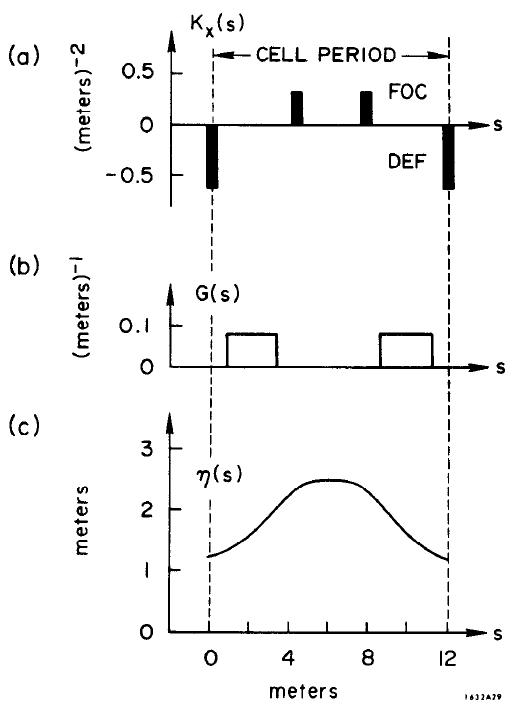
\includegraphics[width=0.6\linewidth]{./Figuras/fig29.jpeg}
	\caption{Funções do campo guia e a função de dispersão. Retirado de \cite{sands1970physics}.}
	\label{fig:fig29}
\end{figure}

Numa seção livre de campo, tanto $G$ quanto $K_x$ são nulas, então $\eta(s)$ tem um segmento com inclinação constante. Num quadrupolo puro, $G$ é zero e $K_x$ é apenas a força do quadrupolo. Num quadrupolo focalizador, $K_x$ é positivo e $\eta(s)$ segue uma oscilação senoidal em torno de zero na forma
\begin{align}
	\eta = a\ cos\left(\sqrt{K_x}s + \vartheta\right)
\end{align}
Em um quadrupolo desfocalizador, $K_x$ é negativo e $\eta(s)$ segue uma exponencial positiva na forma
\begin{align}
	\eta = a\ e^{(\sqrt{-K_x}s + \vartheta)}
\end{align}
A curva de $\eta(s)$ é "atraída" para o eixo $s$ em um quadrupolo focalizador e repelida do eixo em um quadrupolo desfocalizador.

Apesar de $K_1$ ser zero em um dipolo, $K_x$ não é. Na verdade, $K_x=G^2$ e a equação para $\eta$ fica
\begin{align}
	\eta'' = -G^2\eta + G = -G^2\left(\eta - \frac{1}{G}\right)
\end{align}

A curva de $\eta$ é um segmento senoidal o qual é "atraído" para $\eta_0 = 1/G$ com uma "força restauradora" proporcional a $G^2$ ($\eta_0$ é igual ao raio de curvatura $\rho$ da órbita ideal).

Da discussão acima, pode-se entender as características qualitativas das variações de $\eta(s)$ representadas na \autoref{fig:fig29}. Para todos os anéis de armazenamento "normais", a função de dispersão é positiva em todo o anel.

Considerando um campo guia de função separável, pode-se expandir a discussão anterior para calcular $\eta(s)$. Suponha que o cálculo inicie em $s=0$ assumindo alguns valores para $\eta(0)$ e $\eta'(0)$ e $\eta$ seja avaliada como uma sucessão de segmentos do tipo descrito anteriormente, até que seja feita uma revolução completa --  ou seja, até $s=L$. A verdadeira $\eta(s)$ será obtida se $\eta(0)$ e $\eta'(0)$ forem escolhidos de forma que $\eta(0) = \eta(L)$ e $\eta'(0) = \eta'(L)$. O cálculo pode ser computado utilizando uma técnica matricial.

A função de dispersão também pode ser obtida (para qualquer tipo de campo) utilizando os resultados obtidos na \autoref{sec:2.10} para as órbitas fechadas com distúrbio. Pode-se imaginar que a órbita fechada causada pela variação de energia é apenas uma órbita fechada com distúrbio, uma vez que tanto o desvio de energia quanto o erro de campo causam uma mudança na curvatura da trajetória. Em outras palavras, um erro de campo $\delta G$ em um segmento de órbita $\Delta s$ produz uma mudança na curvatura da trajetória de um elétron com energia $E_0$, mudança esta que é a mesma mudança na curvatura resultante de um desvio de energia $\epsilon$ de um elétron que viaja ao longo do campo nominal, já que $\delta G/G = \epsilon/E_0$. Já que $\eta(s)$ é a taxa do desvio da órbita fechada para $\epsilon/E_0$, pode-se computar $\eta(s)$ substituindo $\delta G$ na equação \eqref{eq:2.92} da \autoref{sec:2.11} por $G$. Este argumento também pode ser justificado notando que a equação \eqref{eq:3.4} para $\eta$ tem a mesma forma da equação \eqref{eq:2.85} para $x_c$ na \autoref{sec:2.10}; informalmente pode-se substituir $x_c \rightarrow \eta$ e $\delta G \rightarrow -G$. Fazendo estas substituições na equação \eqref{eq:2.94}, tem-se
\begin{align}
	\eta(s) = \frac{\sqrt{\beta(s)}}{2sen(\pi\nu)}\int\limits_{0}^{L}G(\bar{s})\sqrt{\beta(\bar{s})}cos(|\varphi(s)-\varphi(\bar{s})|-\pi\nu)d\bar{s}
\end{align}
Então, se $\beta(s)$ já é conhecido, pode-se obter $\eta(s)$ por uma integração. Note que $\eta(s)$ também terá um comportamento ressonante quando $\nu$ se aproxima de um inteiro.

Se a órbita ideal não está em um plano, esta discussão deve ser repetida para os desvios verticais. Neste caso, existirão duas funções de curvatura $G_x$ e $G_z$ assim como duas funções de focalização $K_x$ e $K_z$. Os desvios verticais também terão contribuições relativas ao desvio de energia, as quais serão proporcionais a função de dispersão $\eta_z(s)$. E a função de dispersão vertical pode ser avaliada em termos das funções de focalização e curvatura verticais. Terá apenas uma diferença qualitativa importante do caso horizontal: $\eta_z(s)$ terá tanto valores positivos quanto negativos, e sua média ao redor do anel será zero.
	\subsection{Tamanho da órbita: compactação de momento}\label{sec:3.2}
\begin{align}
	\mean{\eta}_{mag} = \frac{1}{\ell_{mag}}\int\limits_{mag}^{}\eta(s)ds\label{eq:3.13}
\end{align}
\begin{align}
	\alpha = \frac{2\pi}{L}\mean{\eta}_{mag} = \frac{\mean{\eta}_{mag}}{R}\label{eq:3.14}
\end{align}
\begin{align}
	\frac{\delta T}{T_0} = \frac{\delta \ell_\epsilon}{L} = \alpha \frac{\epsilon}{E_0}\label{eq:3.15}
\end{align}

%\chapter{Oscilações em Energia}
%\chapter{Amortecimento por Radiação}
%\chapter{Excitação por Radiação}


% Our bibtex file :)
\newpage
\bibliography{biblio}


\end{document}








